%!TEX root = ../terrainbook.tex

\graphicspath{{dtvd/}}


\newcommand{\Orient}{O\textsc{rientation}\xspace}
\newcommand{\walk}{W\textsc{alk}\xspace}
\newcommand{\Insphere}{I\textsc{n}C\textsc{ircle}\xspace}




\chapter{Triangulations \& Voronoi diagrams}



\section{The Voronoi Diagram}

Let $S$ be a set of points in $\mathbb{R}^2$ (the two-dimensional Euclidean space). 
The Voronoi cell of a point $p \in S$, defined $\mathcal{V}_{p}$, is the set of points $x \in \mathbb{R}^2$ that are closer to $p$ than to any other point in $S$; that is:
\begin{equation}
\mathcal{V}_p = \{x \in \mathbb{R}^{2} \ | \ \|x-p\| \, \leq \, \|x-q\|, \ \forall \, q \in S \}. 
\end{equation}
The union of the Voronoi cells of all generating points $p \in S$ form the Voronoi diagram of $S$, defined VD($S$). 
If $S$ contains only two points $p$ and $q$, then VD($S$) is formed by a single line defined by all the points $x \in \mathbb{R}^2$ that are equidistant from $p$ and $q$. 
This line is the perpendicular bisector of the line segment from $p$ to $q$, and splits the plane into two half-planes. 
$\mathcal{V}_p$ is formed by the half-plane containing $p$, and $\mathcal{V}_q$ by the one containing $q$. 
As shown in Figure~\ref{fig:halfspaces}a,
\begin{figure}
  \centering
  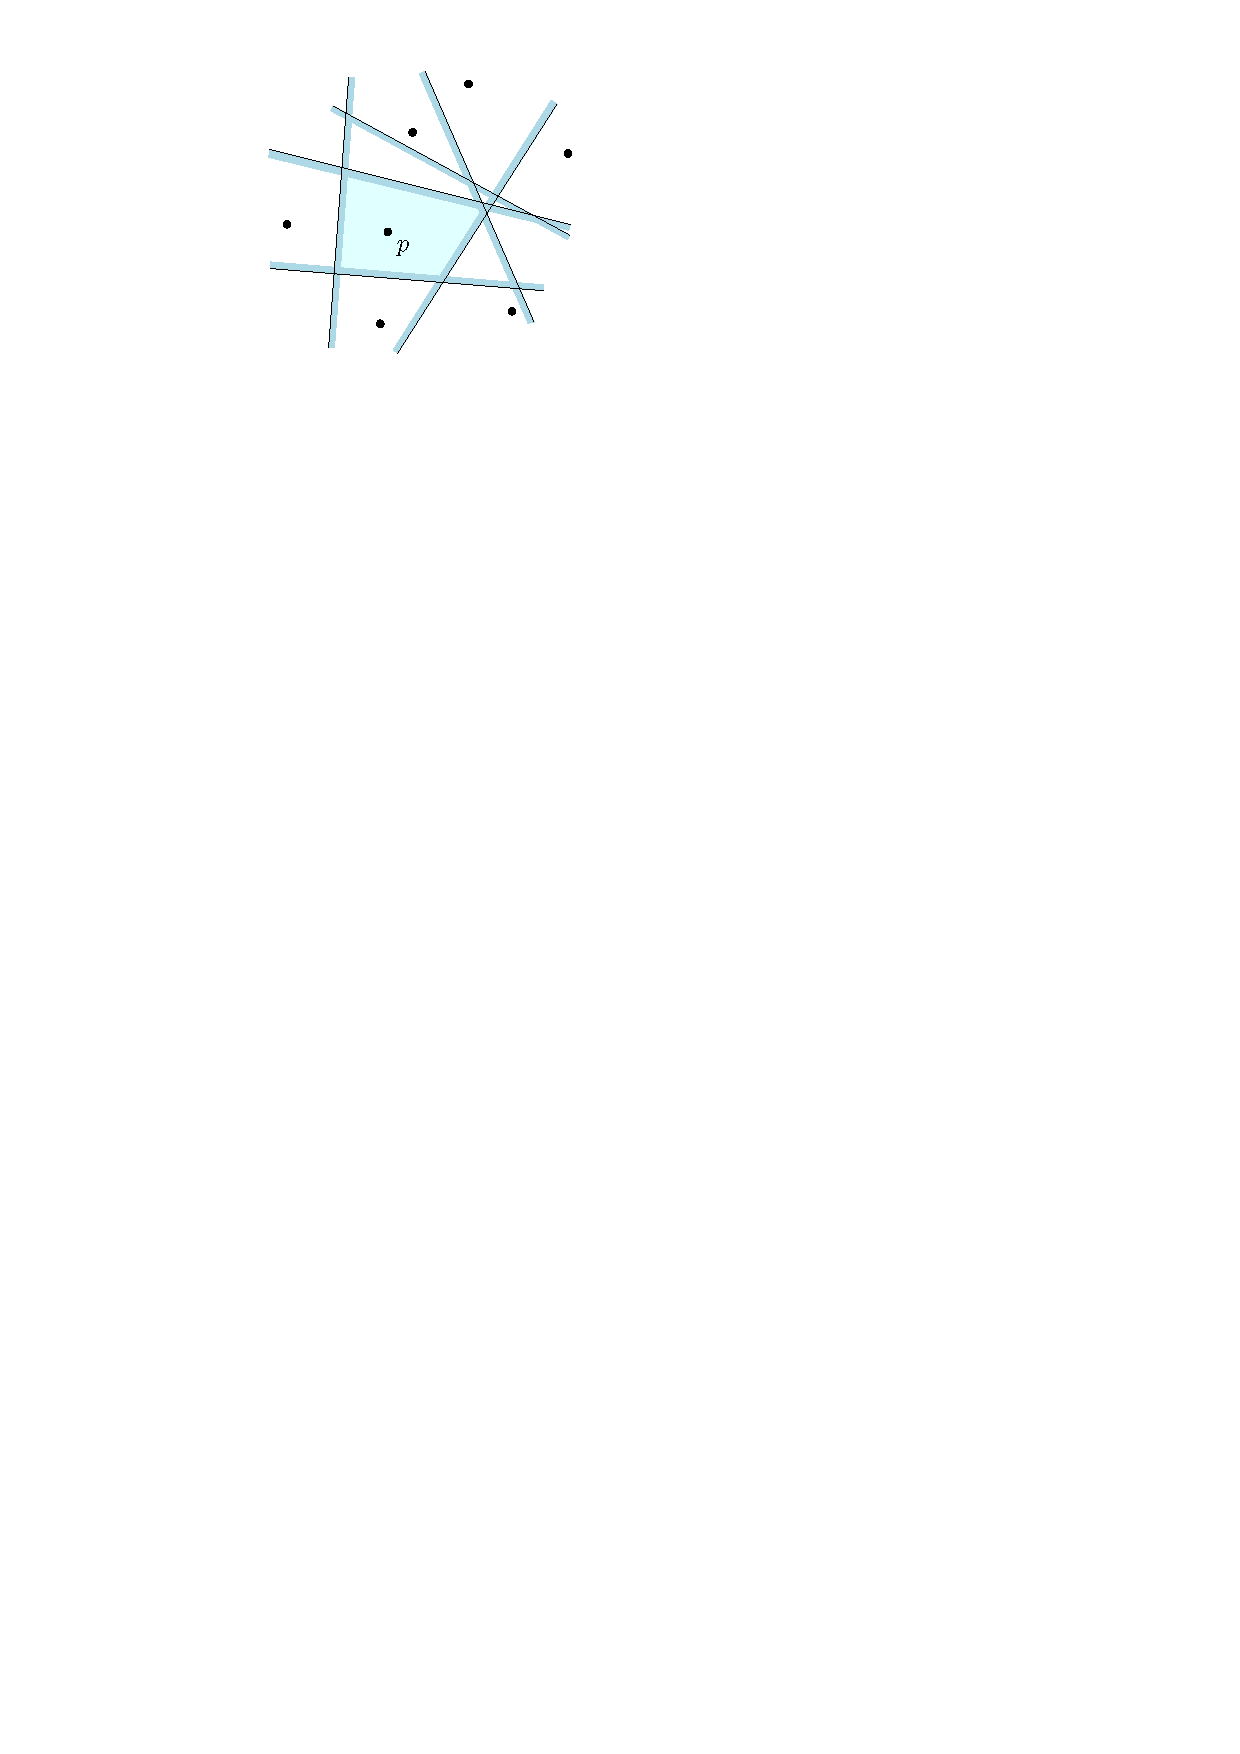
\includegraphics[width=0.6\textwidth]{figs/halfspaces}
  \caption{\textbf{(a)} The Voronoi cell $\mathcal{V}_p$ is formed by the intersection of all the half-planes between $p$ and the other points. \textbf{(b)} The VD for a set $S$ of points in the plane (the black points). The Voronoi vertices (white points) are located at the centre of the circle passing through three points in $S$, provided that this circle contains no other points in $S$ in its interior.} 
\label{fig:halfspaces}
\end{figure}
when $S$ contains more than two points (let us say it contains $n$ points), the Voronoi cell of a given point $p \in S$ is obtained by the intersection of $n-1$ half-planes defined by $p$ and the other points $q \in S$. 
That means that $\mathcal{V}_{p}$ is always convex. 
Notice also that every point $x \in \mathbb{R}^2$ has at least one nearest point in $S$, which means that VD($S$) covers the entire space.

%

As shown in Figure~\ref{fig:halfspaces}b, the VD of a set $S$ of points in $\mathbb{R}^2$ is a planar graph. 
Its edges are the perpendicular bisectors of the line segments of pairs of points in $S$, and its vertices are located at the centres of the circles passing through three points in $S$. 
The VD in $\mathbb{R}^2$ can also be seen as a two-dimensional cell complex where each 2-cell is a (convex) polygon (see Figure~\ref{fig:vd2d}). 
\begin{figure}
  \centering
  \includegraphics[page=3,width=0.6\textwidth]{figs/vd2d}
  \caption{VD of a set of points in the plane (clipped by a box). The point $p$ (whose Voronoi cell is dark grey) has seven neighbouring cells (light grey).} 
\label{fig:vd2d}
\end{figure}
Two Voronoi cells, $\mathcal{V}_{p}$ and $\mathcal{V}_{q}$, lie on the opposite sides of the perpendicular bisector separating the points $p$ and $q$. 

%

The VD has many interesting properties, what follows is a list of the most relevant properties in the context of this course.
\begin{description}
  \item[Size:] if $S$ has $n$ points, then VD($S$) has exactly $n$ Voronoi cells since there is a one-to-one mapping between the points and the cells.
  \item[Voronoi vertices:] a Voronoi vertex is equidistant from 3 data points. Observe for instance in Figure~\ref{fig:halfspaces}b that the Voronoi vertices are at the centre of circles.
  \item[Voronoi edges:] a Voronoi edge is equidistant from 2 points.
  \item[Convex hull:] let $S$ be a set of points in $\mathbb{R}^2$, and $p$ one of its points. $\mathcal{V}_{p}$ is unbounded if $p$ bounds conv($S$). Otherwise, $\mathcal{V}_{p}$ is the convex hull of its Voronoi vertices. Observe that in Figure~\ref{fig:halfspaces}b, only the point in the middle has a bounded Voronoi cell.
\end{description}
  

%%%
%
\section{The Delaunay Triangulation}
\label{sec:dt_definition}

Let $\mathcal{D}$ be the VD of a set $S$ of points in $\mathbb{R}^2$. 
Since VD($S$) is a planar graph, it has a dual graph, and let $\mathcal{T}$ be this dual graph obtained by drawing straight edges between two points $p,q \in S$ if and only if $\mathcal{V}_{p}$ and $\mathcal{V}_{q}$ are adjacent in $\mathcal{D}$. 
Because the vertices in $\mathcal{D}$ are of degree 3 (3 edges connected to it), the graph $\mathcal{T}$ is a triangulation. 
$\mathcal{T}$ is actually called the Delaunay triangulation (DT) of $S$, and, as shown in Figure~\ref{fig:dt2da}, 
\begin{figure}
  \centering
  \begin{subfigure}[b]{0.45\linewidth}
    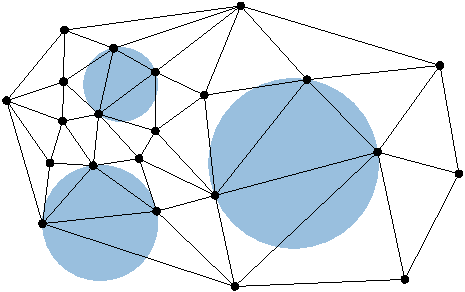
\includegraphics[width=\textwidth]{figs/dt2d_2}
    \caption{}\label{fig:dt2da}
  \end{subfigure}%
  \qquad
  \begin{subfigure}[b]{0.3\linewidth}
    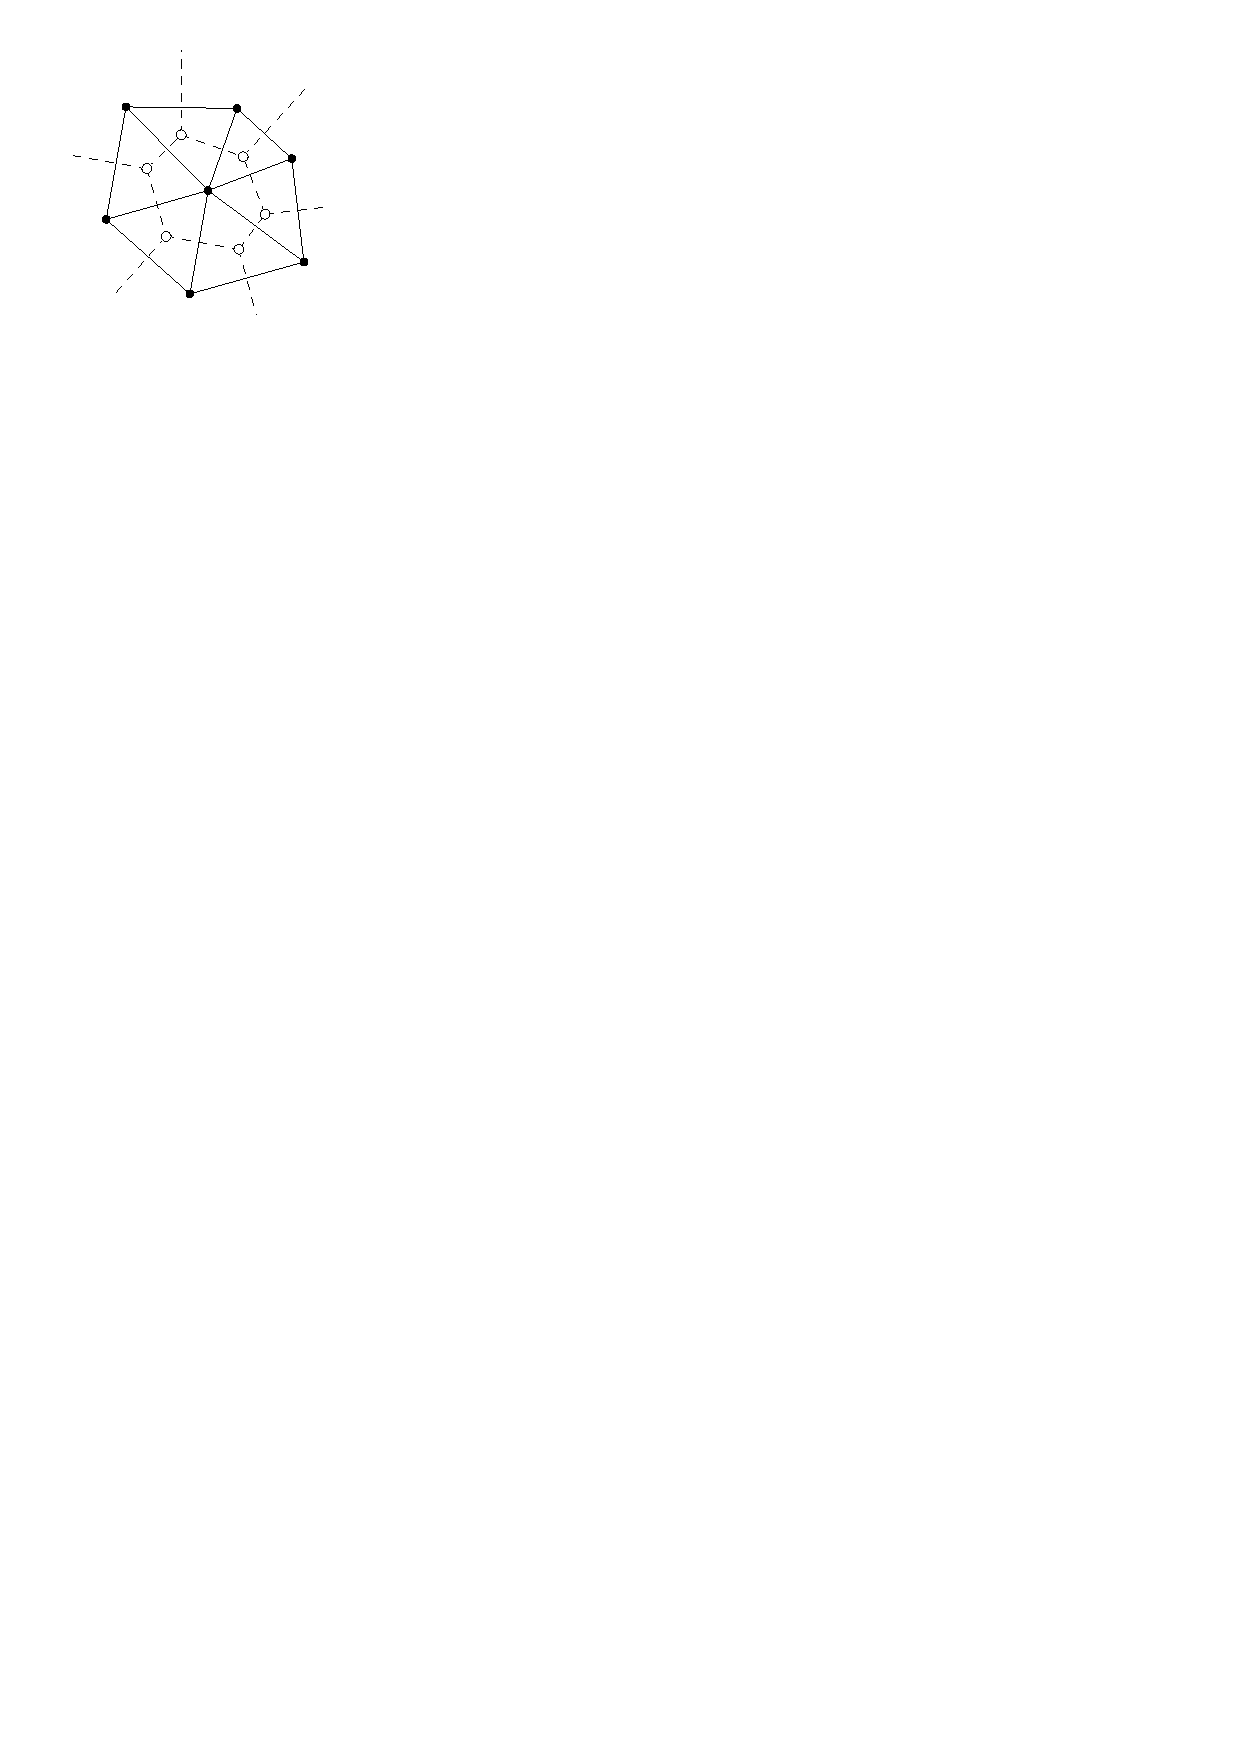
\includegraphics[width=\textwidth]{figs/duality_2d}
    \caption{}\label{fig:dt2db}
  \end{subfigure}%
  \caption{\textbf{(a)} The DT of a set of points in the plane (same point set as Figure~\ref{fig:vd2d}). \textbf{(b)} Both the DT (black lines) and the VD (dashed lines) of a set of points in the plane.}
\label{fig:dt2d}
\end{figure}
partitions the plane into triangles---where the vertices of the triangles are the points in $S$ generating each Voronoi cell---that satisfy the \emph{empty circumcircle} test (a circle is said to be \emph{empty} when no points are in its interior). 
If $S$ is in general position, then DT($S$) is unique.

%
\subsection{Convex Hull}
The DT of a set $S$ of points subdivides completely conv($S$), \ie\ the union of all the triangles in DT($S$) is conv($S$).

Let $S$ be a set of points in $\mathbb{R}^2$, the \emph{convex hull} of $S$, denoted conv($S$), is the minimal convex set containing $S$. 
It is best understood with the elastic band analogy: imagine each point in $\mathbb{R}^2$ being a nail sticking out of the plane, and a rubber band stretched to contain all the nails, as shown in Figure~\ref{fig:convex_hull}. 
\begin{figure}
  \centering
  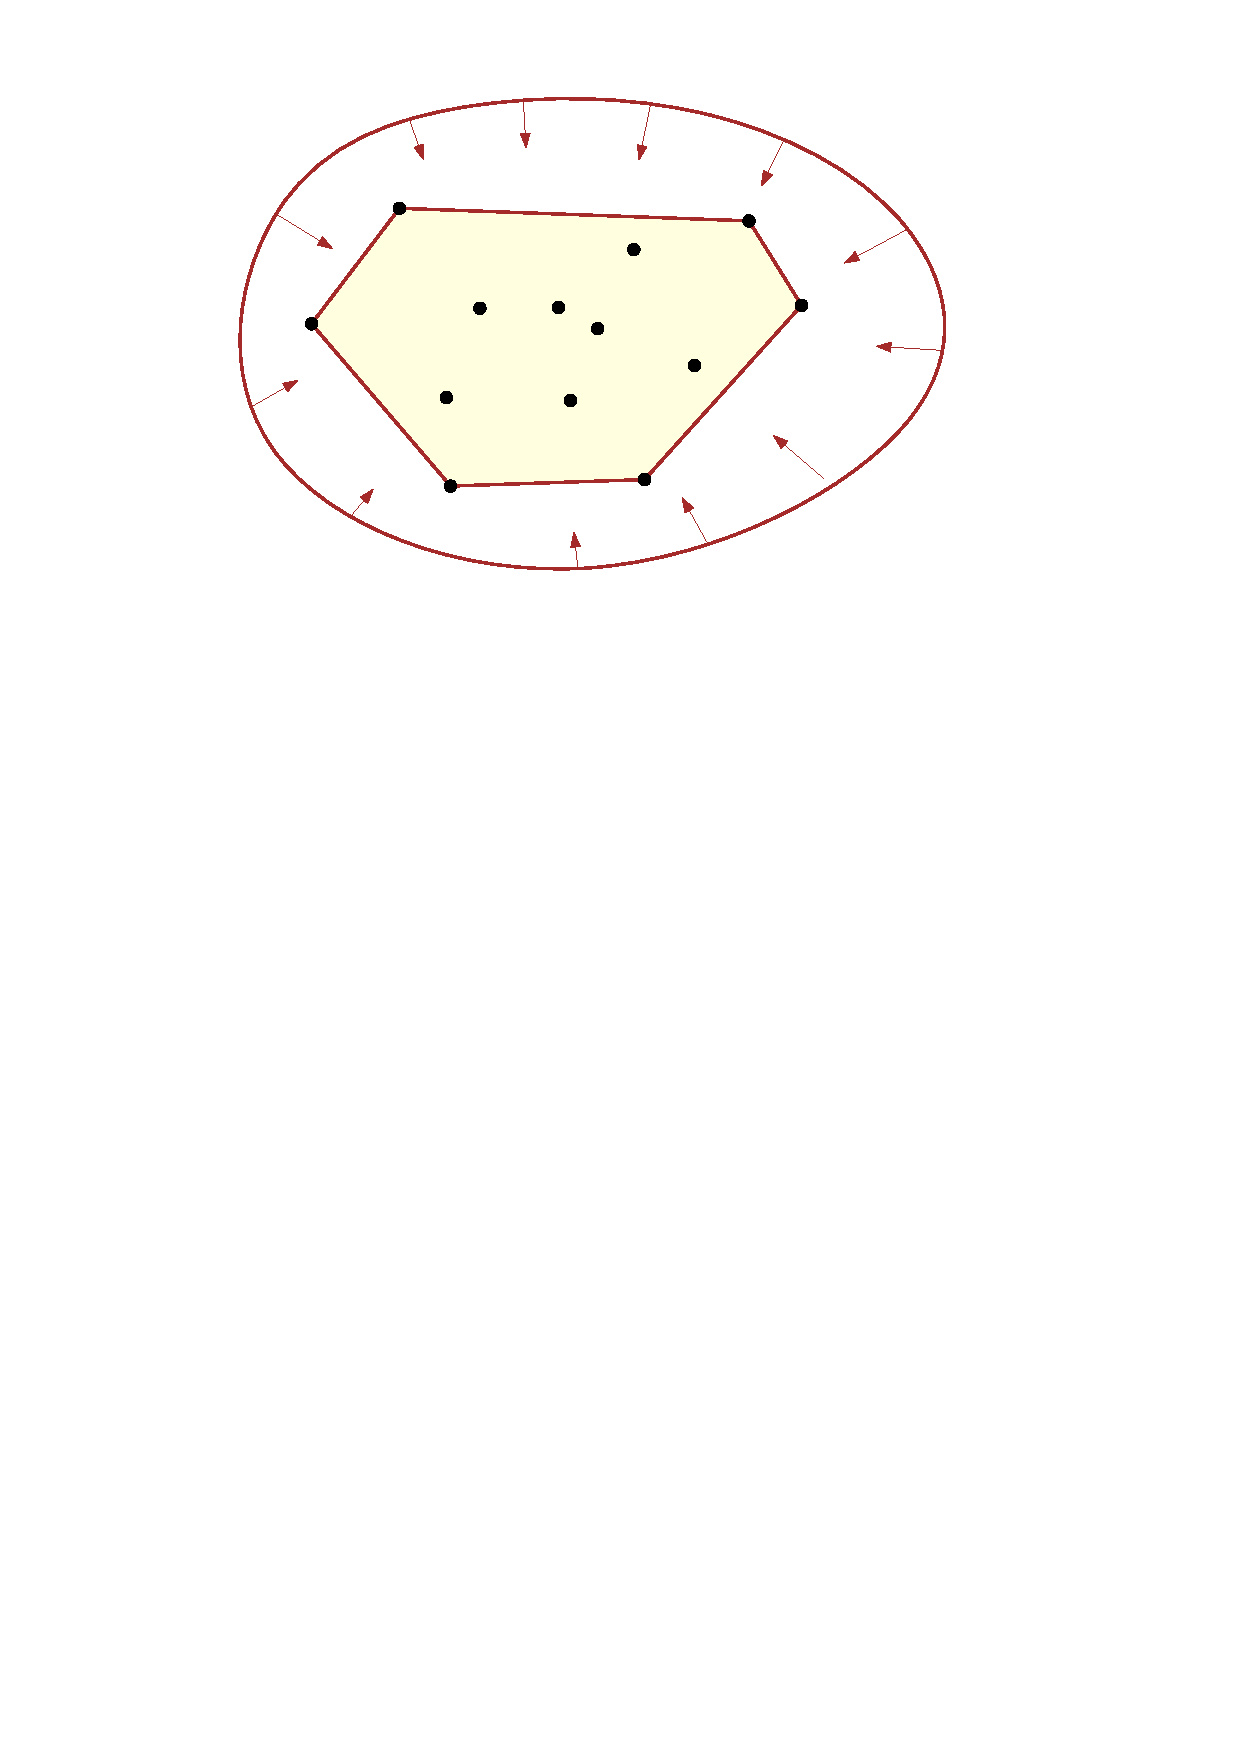
\includegraphics[width=0.35\textwidth]{figs/convex_hull}
  \caption{The convex hull of a set of points in $\mathbb{R}^2$.} 
\label{fig:convex_hull}
\end{figure}
When released, the rubber band will assume the shape of the convex hull of the nails. 
Notice that conv($S$) is not only formed by the edges connecting the points (the rubber band), but all the points of $\mathbb{R}^2$ that are contained within these edges (thus the whole polygon).


%
\subsection{Local Optimality}
Let $\mathcal{T}$ be a triangulation of $S$ in $\mathbb{R}^2$. 
An edge $\sigma$ is said to be \emph{locally} Delaunay if it either:
\begin{description}
  \item[(i)] belongs to only one triangle, and thus bounds conv($S$), or
  \item[(ii)] belongs to two triangles $\tau_a$ and $\tau_b$, formed by the vertices of $\sigma$ and respectively the vertices $p$ and $p$, and $p$ is outside of the circumcircle of $\tau_a$. 
\end{description}
The second case is illustrated in Figure~\ref{fig:local}: the triangles $abd$ and $bcd$ are Delaunay, and thus is the edge $bd$; the edge $ac$ is not Delaunay.
\begin{figure}
  \centering
  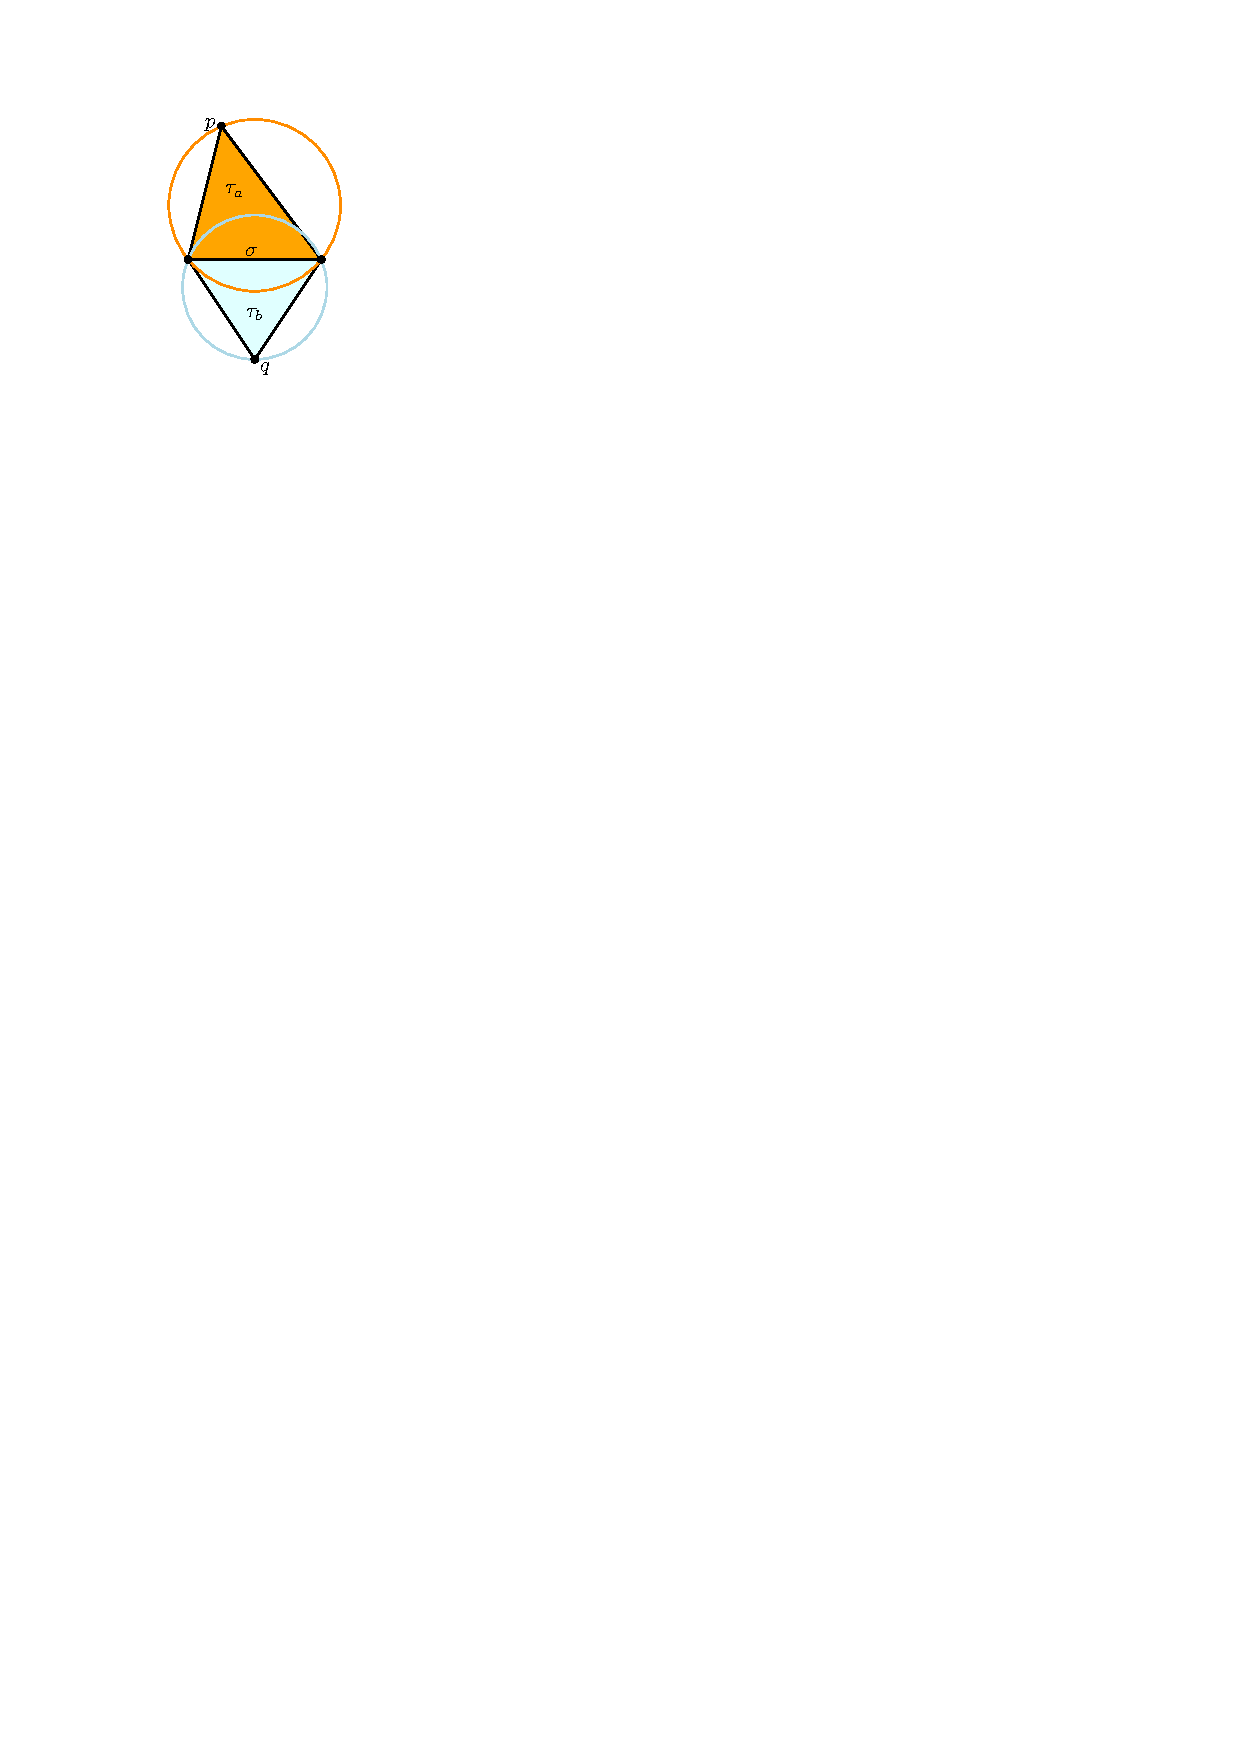
\includegraphics[width=0.7\textwidth]{figs/local}
  \caption{Only one configuration is Delaunay (the left one).} 
\label{fig:local}
\end{figure}
In an arbitrary triangulation, not every edge that is locally Delaunay is necessarily a edge of DT($S$), but local optimality implies globally optimality in the case of the DT:
\begin{quote}
  Let $\mathcal{T}$ be a triangulation of a point set $S$ in $\mathbb{R}^2$. If every edge of $\mathcal{T}$ is locally Delaunay, then $\mathcal{T}$ is the Delaunay triangulation of $S$.
\end{quote}
This has serious implications as the DT---and its dual---are locally modifiable, \ie\ we can theoretically insert, delete or move a points in $S$ without recomputing DT($S$) from scratch.


%%%
%
\subsection{Angle Optimality}
The DT in two dimensions has a very important property that is useful in applications such as finite element meshing or interpolation: the \emph{max-min angle optimality}. Among all the possible triangulations of a set $S$ of points in $\mathbb{R}^2$, DT($S$) maximises the minimum angle (max-min property), and also minimises the maximum circumradii. 
In other words, it creates triangles that are as equilateral as possible. 
Notice here that maximising the minimum angle is not the same as minimising the maximum, and the DT only guarantees the former.


%%%
\subsection{Lifting on the paraboloid}
\label{sec:parabolic_lifting}

There exists a close relationship between DTs in $\mathbb{R}^{d}$ and convex polytopes in $\mathbb{R}^{d+1}$. 

Let $S$ be a set of points in $\mathbb{R}^{d}$, and let $x_{1}, x_{2}, \ldots , x_{d}$ be the coordinates axes. 
The parabolic lifting map projects each vertex $v(v_{x1}, v_{x2}, \ldots , v_{xd})$ to a vertex $v^{+}(v_{x1}, v_{x2}, \ldots , v_{xd}, v_{x1}^{2}+v_{x2}^{2}+\cdots+v_{xd}^{2})$ on the paraboloid of revolution in $\mathbb{R}^{d+1}$. 
The set of points thus obtained is denoted $S^{+}$. 
Observe that, for the two-dimensional case, the paraboloid in three dimensions defines a surface whose vertical cross sections are parabolas, and whose horizontal cross sections are circles; the same ideas are valid in higher dimensions. 

%

The relationship is the following: every facet (a $d$-dimensional simplex) of the lower envelope of conv($S^{+}$) projects to a $d$-simplex of the Delaunay triangulation of $S$. 
This is illustrated in Figure~\ref{fig:paraboloid} for the construction of the DT in $\mathbb{R}^{2}$. 
\begin{figure}
  \centering
  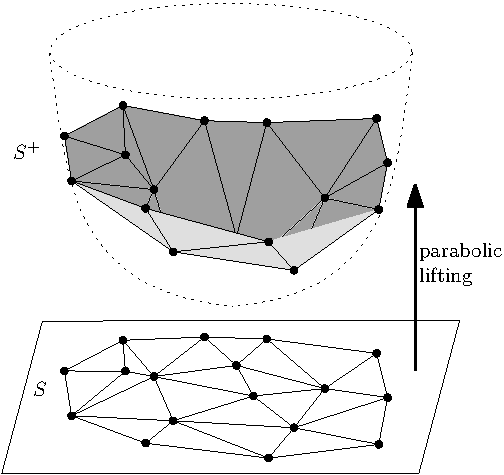
\includegraphics[width=0.4\textwidth]{figs/paraboloid}
  \caption{The parabolic lifting map for a set $S$ of points $\mathbb{R}^2$.}
\label{fig:paraboloid}
\end{figure}

%

In short, the construction of the $d$-dimensional DT can be transformed into the construction of the convex hull of the lifted set of points in ($d+1$) dimensions.
In practice, since it is easier to construct convex hulls (especially in higher dimensions, \ie\ 4+), the DT is often constructed with this method.




%%%
%
\subsection{Degeneracies}
\label{sec:degeneracies}

The previous definitions of the VD and the DT assumed that the set $S$ of points is in general position, \ie\ the distribution of points does not create any ambiguity in the two structures. 
For the VD/DT in $\mathbb{R}^{2}$, the degeneracies, or special cases, occur when 3 points lie on the same line and/or when 4 points are cocircular. 
For example, in two dimensions, when four or more points in $S$ are cocircular there is an ambiguity in the definition of DT($S$). 
As shown in Figure~\ref{fig:degeneracies},
\begin{figure}
  \centering
  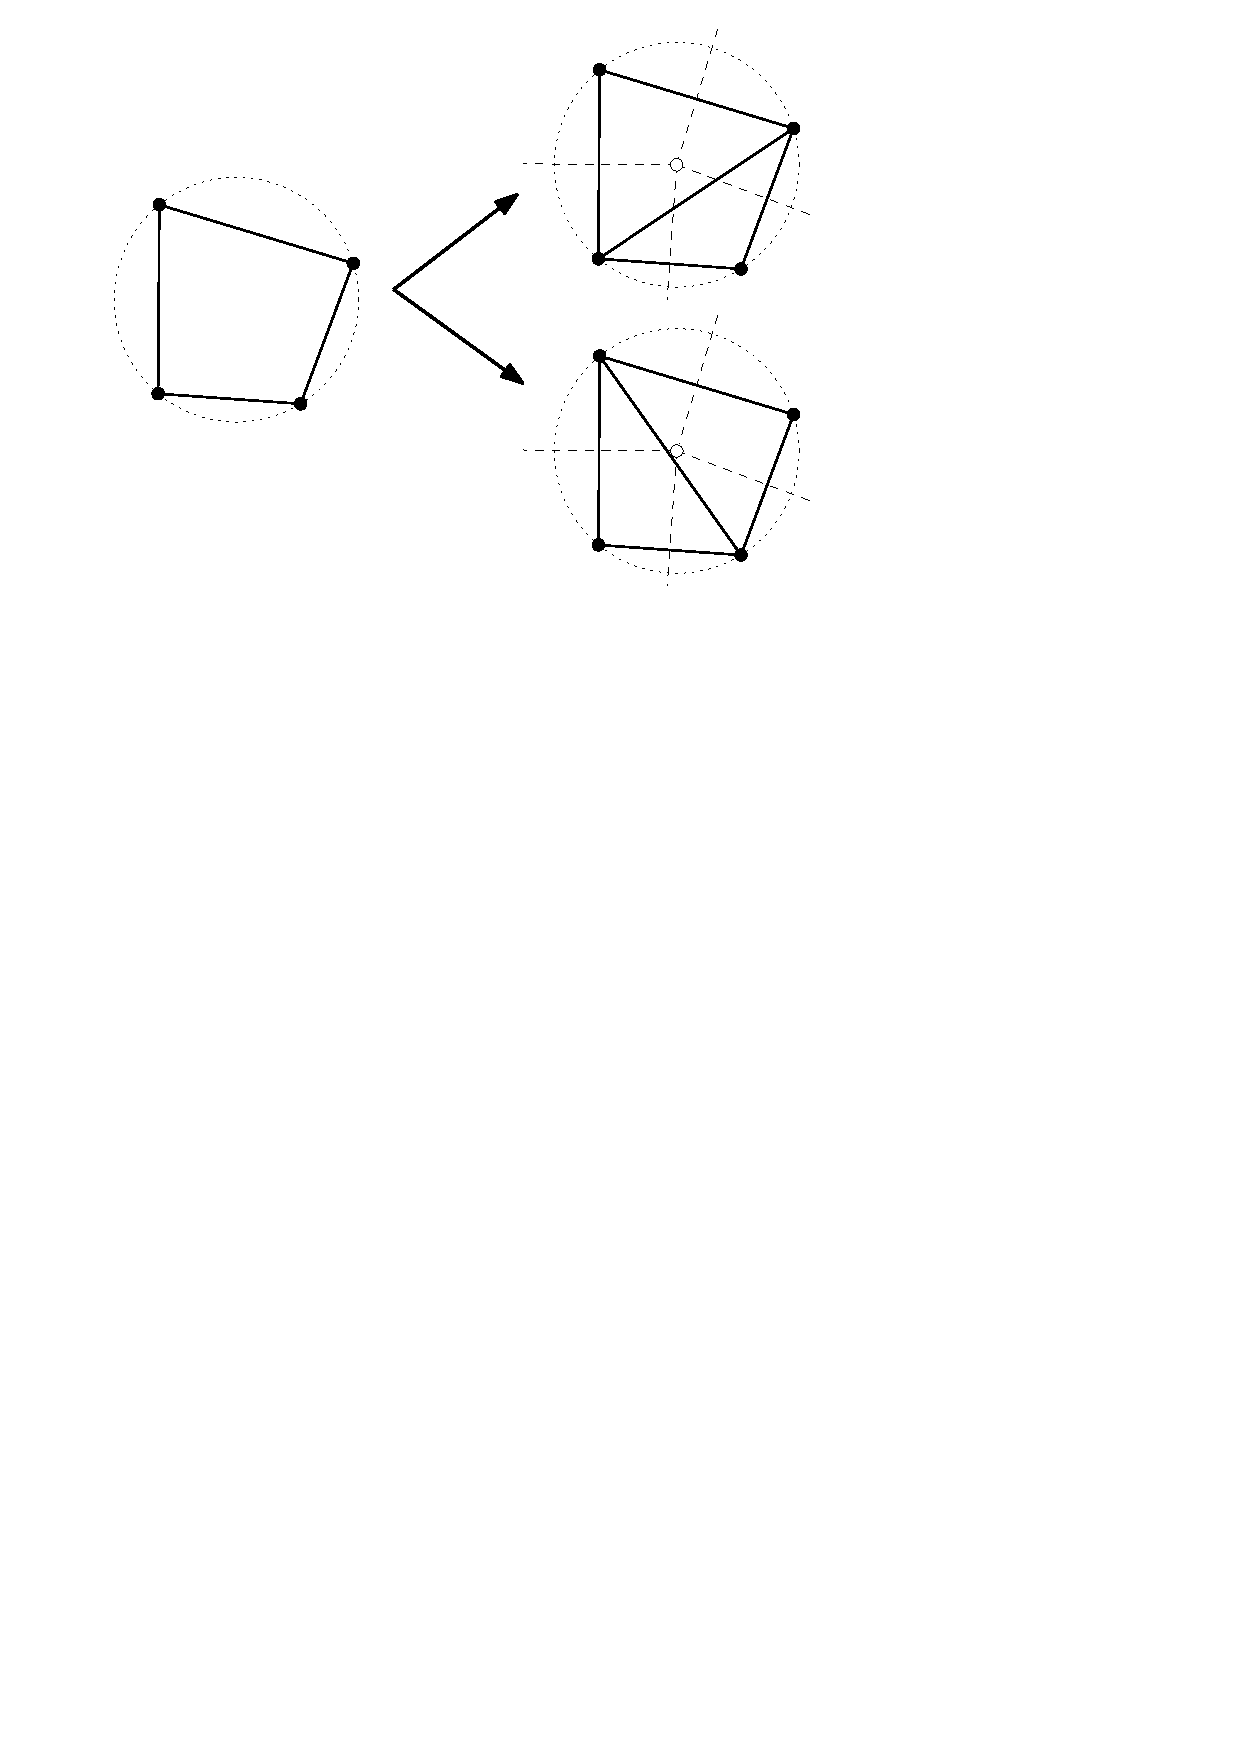
\includegraphics[width=0.4\textwidth]{figs/degeneracies}
  \caption{The DT for four cocircular points in two dimensions is not unique (but the VD is).}
\label{fig:degeneracies}
\end{figure}
the quadrilateral can be triangulated with two different diagonals, and an arbitrary choice must be made since both respect the Delaunay criterion (points should not be on the interior of a circumcircle, but more than three can lie directly on the circumcircle).

This implies that in the presence of four or more cocircular points, DT($S$) is not unique. 
Notice that even in the presence of cocircular points, VD($S$) is still unique, but it has different properties. 
For example, in Figure~\ref{fig:degeneracies}, the Voronoi vertex in the middle has degree 4 (remember that when $S$ is in general position, every vertex in VD($S$) has degree 3). 
When three or more points are collinear, DT($S$) and VD($S$) are unique, but problems with the implementation of the structures can arise.


%%%
%
\section{Duality between the DT and the VD}
\label{sec:duality}

Duality can have many different meanings in mathematics, but it always refers to the translation or mapping in a one-to-one fashion of concepts or structures. 
We use it in this course in the sense of the dual graph of a given graph. 
Let $G$ be a planar graph, as illustrated in Figure~\ref{fig:dual_graph} (black edges).
\begin{figure}
  \centering
  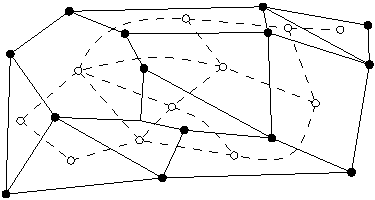
\includegraphics[width=0.45\textwidth]{figs/dual_graph}
  \caption{A graph $G$ (black lines), and its dual graph $G^\star$ (dashed lines).}
\label{fig:dual_graph}
\end{figure}
Observe that $G$ can also be seen as a cell complex in $\mathbb{R}^{2}$. 
The duality mapping is as follows (also shown in details in Figure~\ref{fig:dualdetailtab})
The dual graph $G^{\star}$ has a vertex for each face (polygon) in $G$, and the vertices in $G^{\star}$ are linked by an edge if and only if the two corresponding dual faces in $G$ are adjacent (in Figure~\ref{fig:dual_graph}, $G^{\star}$ is represented with dashed lines). 
Notice also that each polygon in $G^{\star}$ corresponds to a vertex in $G$, and that each edge of $G$ is actually dual to one edge (an arc in Figure~\ref{fig:dual_graph}) of $G^{\star}$ (for the sake of simplicity the dual edges to the edges on the boundary of $G$ are not drawn).

The VD and the DT are the best example of the duality between plane graphs.

\begin{figure}[h]
% \centering
% \setcapindent{1em}
\centering
\begin{minipage}[c]{0.4\textwidth}
  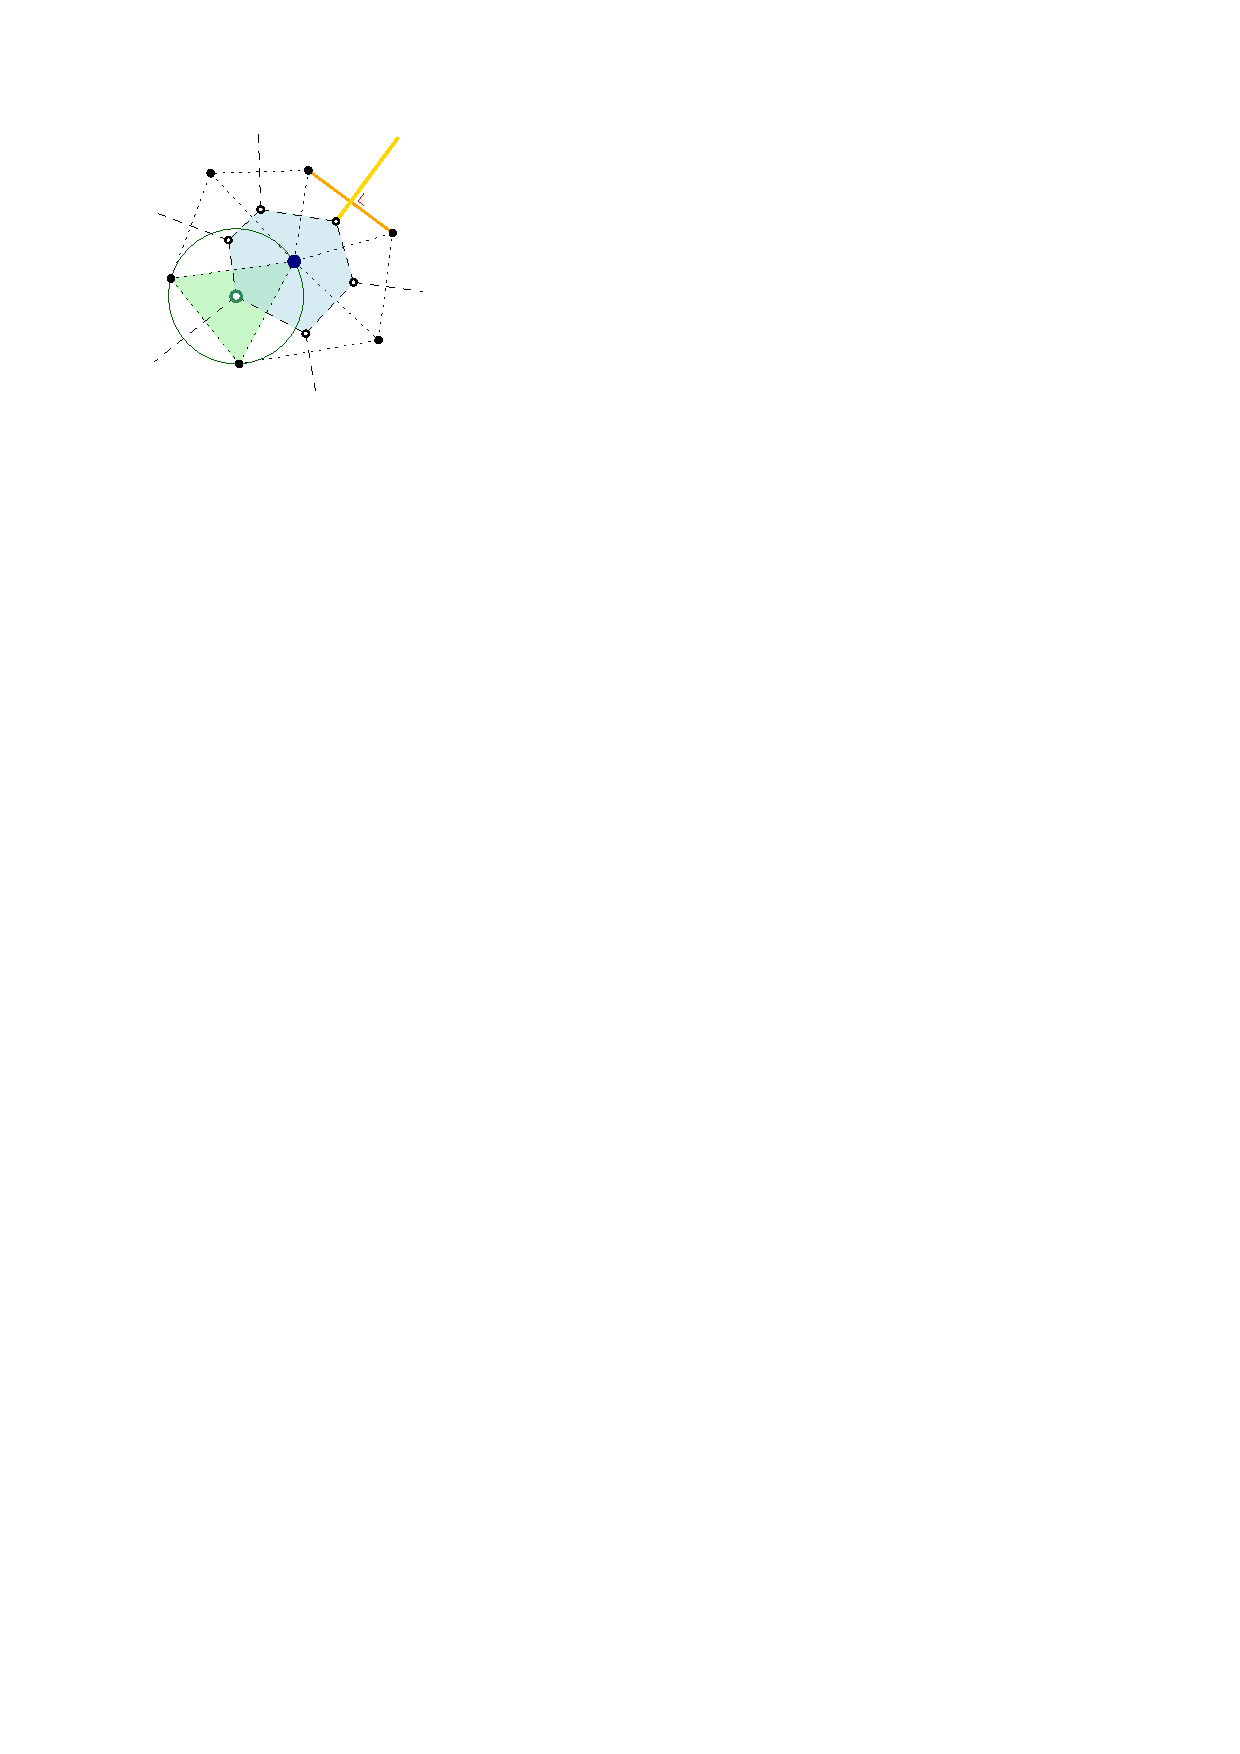
\includegraphics[width=\textwidth]{figs/dualdetail.pdf}
\end{minipage}
\begin{minipage}[c]{0.45\textwidth}
% \hspace{1.1em}
  \centering
  \begin{tabular}{lcl}
  \toprule
  DT & & VD \\
  \midrule
  $\mathbf{\color{YellowGreen}{face}}$ & $\leftrightarrow$ & $\mathbf{\color{ForestGreen}{vertex}}$\\
  $\mathbf{\color{Blue}{vertex}}$ & $\leftrightarrow$ & $\mathbf{\color{SkyBlue}{face}}$\\
  $\mathbf{\color{Orange}{edge}}$ & $\leftrightarrow$ & $\mathbf{\color{Dandelion}{edge}}$\\
  \bottomrule
  \end{tabular}
\end{minipage}
\caption{Duality between the DT (dotted) and the VD (dashed).}
\label{fig:dualdetailtab}
\end{figure}


%%%
%
\section{Incremental construction of the DT}

Since the VD and the DT are dual structures, the knowledge of one implies the knowledge of the other one. 
In other words, if one has only one structure, she can always extract the other one. 
Because it is easier, from an algorithmic and data structure point of view, to manage triangles over arbitrary polygons (they have a constant number of vertices and neighbours), constructing and manipulating a VD by working only on its dual structure is simpler and usually preferred. 
When the VD is needed, it is extracted from the DT\@. 
This has the additional advantage of speeding up algorithms because when the VD is used directly intermediate Voronoi vertices---that will not necessarily exist in the final diagram---need to be computed and stored.

%

While there exists different strategies to construct at DT, we focus here on the \emph{incremental} method (since it is easier to understand and implement).
An incremental algorithm is one where the structure is built incrementally; in our case this means that each point is inserted one at a time in a valid DT and the triangulation is updated, with respect to the Delaunay criterion (empty circumcircle), after each insertion. 
Observe that the insertion of a single point $p$ in a DT modifies only locally the DT, \ie\ only the triangles whose circumcircle contains $p$ need to be deleted and replaced by new ones respecting the Delaunay criterion (see Figure~\ref{fig:insertion_deletion}
\begin{figure}
  \centering
  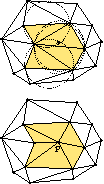
\includegraphics[width=0.6\textwidth]{figs/insertion_deletion}
  \caption{The DT before and after a point $p$ has been inserted. Notice that the DT is updated only locally (only the shaded part of the triangulation is affected).} 
\label{fig:insertion_deletion}
\end{figure}
for an example). 
In sharp contrast to this, other strategies to construct a DT (\eg\ divide-and-conquer and plane sweep algorithms, see Section~\ref{sec:notes}), build a DT in \emph{one} operation (this is a batch operation), and if another point needs to be inserted after this, the whole construction operation must be done again from scratch. 
That hinders their use for some applications where new data coming from a sensor would have to be added.


\begin{figure}
  \centering
  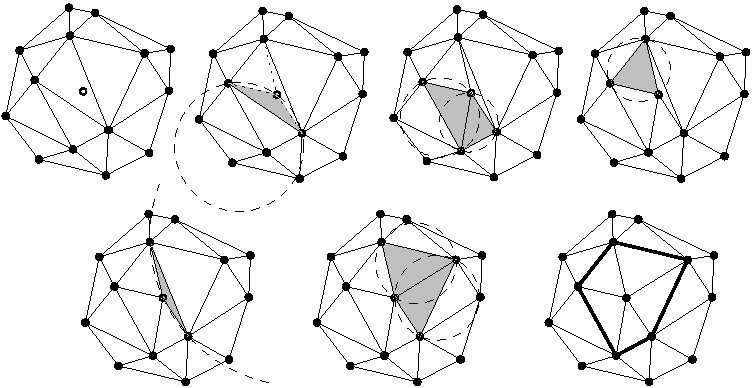
\includegraphics[width=1.0\textwidth]{figs/insertion_steps}
  \caption{Step-by-step insertion, with flips, of a single point in a DT in two dimensions.}
\label{fig:insertion_steps}
\end{figure}
\begin{algorithm}[tb] 
  \KwIn{A DT($S$) $\mathcal{T}$ , and a new point $p$ to insert}
  \KwOut{$\mathcal{T}^{p} = \mathcal{T} \cup \{p\}$ // the DT with point $p$}
  find triangle $\tau$ containing $p$\;
  insert $p$ in $\tau$ by splitting it in to 3 new triangles\;
  push 3 new triangles on a stack\;
  \While{stack is non-empty}
  {
    $\tau = \{p,a,b\} \leftarrow$ pop from stack\;
    $\tau_{a} = \{a,b,c\} \leftarrow$ get adjacent triangle of $\tau$ having the edge $ab$\;
    \If{$c$ is inside circumcircle of $\tau$}
    {
      flip the triangles $\tau$ and $\tau_{a}$\;
      push 2 new triangles on stack\;
    }
  }
  \caption{Algorithm to insert one point in a DT}
\label{algo:insert1pt}
\end{algorithm} 

Figure~\ref{fig:insertion_steps} describes the algorithm, and Algorithm~\ref{algo:insert1pt} its pseudo-code. 
In a nutshell, for the insertion of a new point $p$ in a DT($S$), the triangle $\tau$ containing $p$ is identified and then split into three new triangles by joining $p$ to every vertex of $\tau$. 
Second, each new triangle is tested---according to the Delaunay criterion---against its opposite neighbour (with respect to $p$); if it is not a Delaunay triangle then the edge shared by the two triangles is \emph{flipped} (see below) and the two new triangles will also have to be tested later. 
This process stops when every triangle having $p$ as one of its vertices respects the Delaunay criterion.

%%%
\paragraph{Walk/Point location.} To find the triangle containing the new inserted point $p$, we can use the point-in-polygon test for every triangle (as explained in class), but that would be too slow. 
An better alternative, is to use the adjacency relationships between the triangles, and use the \emph{side} tests as described in the book to navigation from one triangle to the other, until we find the the good one. 
The idea is shown in Figure~\ref{fig:walk}
\begin{figure}
  \centering
  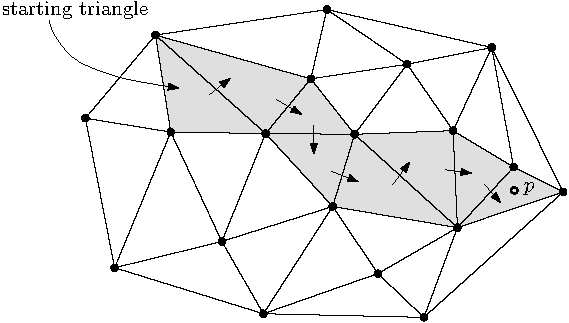
\includegraphics[width=0.5\textwidth]{figs/walk}
  \caption{The Walk algorithm for a DT in two dimensions. The query point is $p$.}
\label{fig:walk}
\end{figure}


%%%
\paragraph{Flips.}The \emph{flip} operation we use to modify the triangulation is a simple local topological operation that modifies the configuration of two adjacent triangles. 
Consider the set $S = \{a, b, c, d\}$ of points in the plane forming a quadrilateral, as shown in Figure~\ref{p:flip22}. 
\begin{figure}
  \centering
  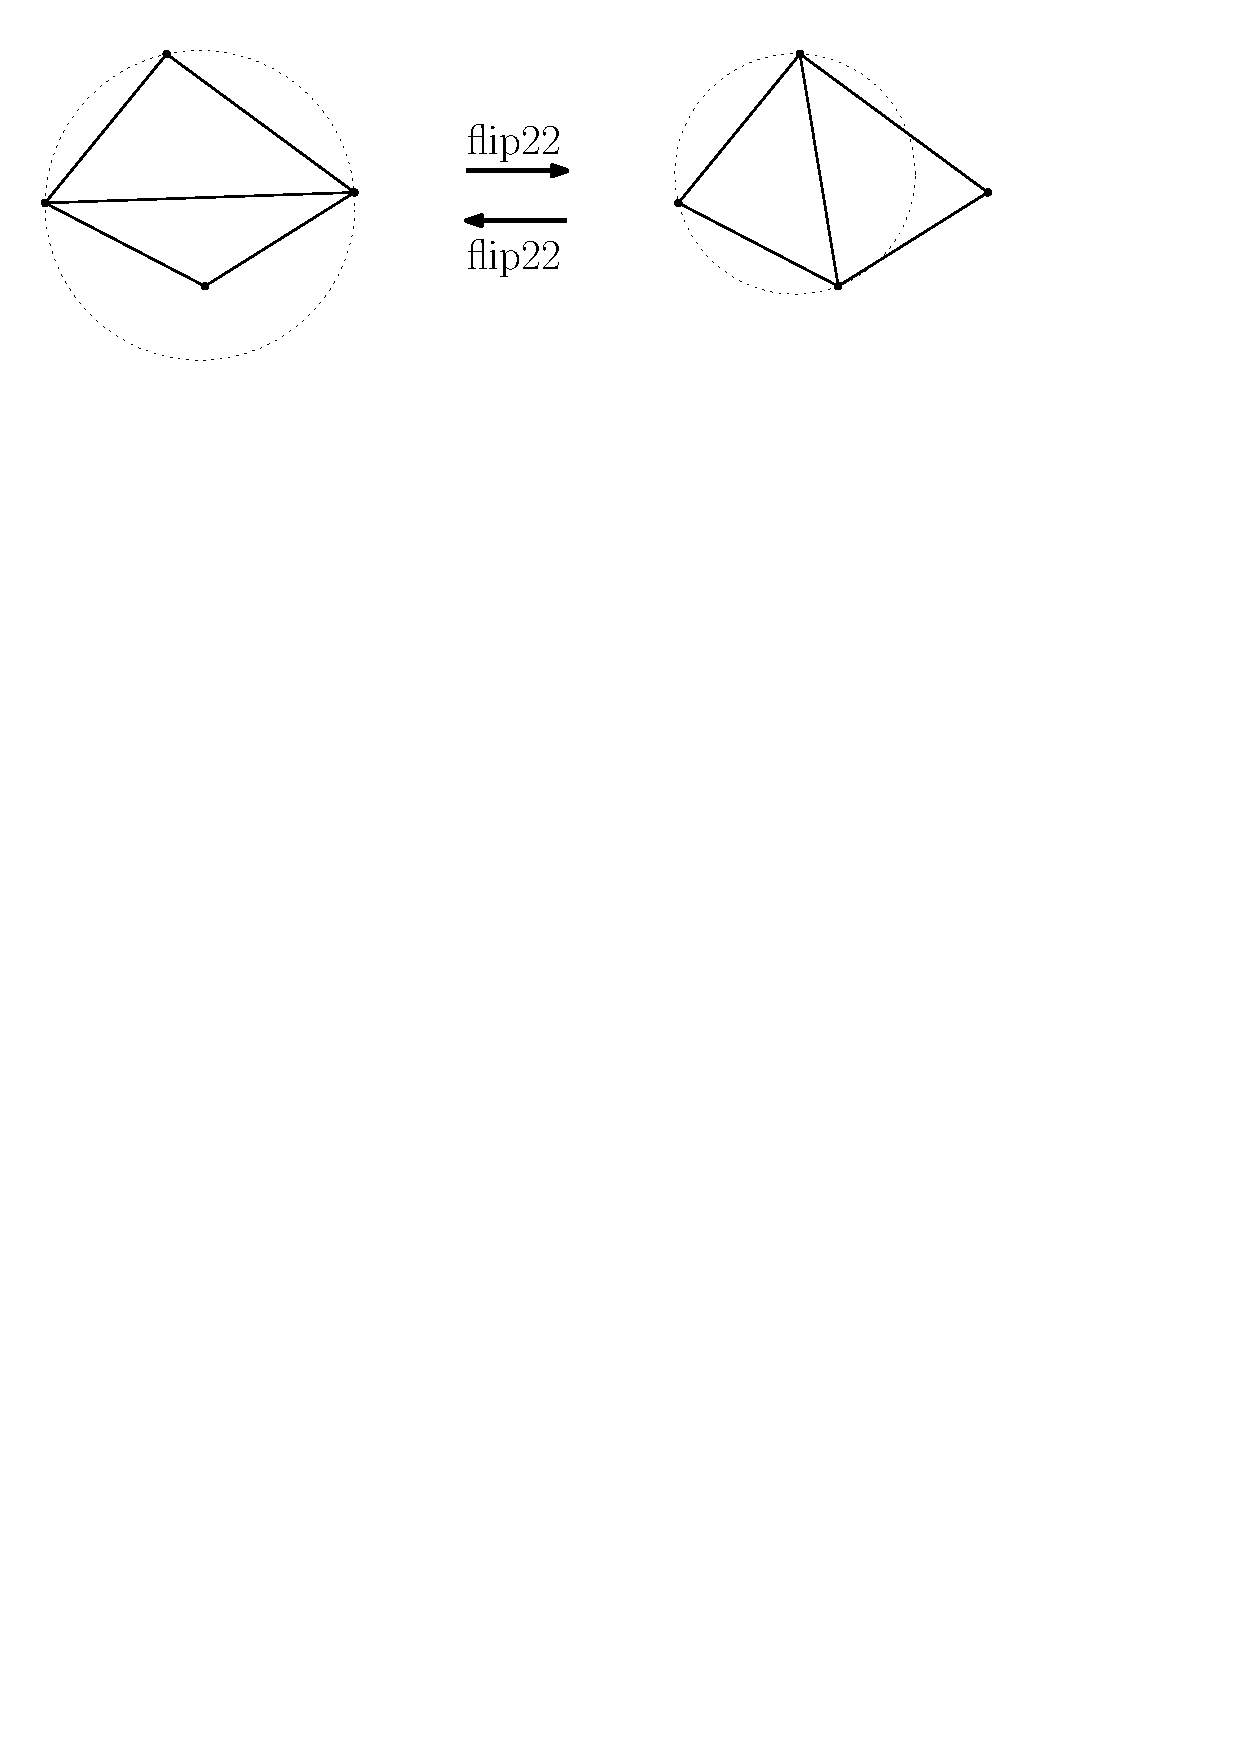
\includegraphics[width=0.5\textwidth]{figs/flip22}
  \caption{A flip22}
\label{p:flip22}
\end{figure}
There exist exactly two ways to triangulate $S$: the first one contains the triangles $abc$ and $bcd$; and the second one contains the triangles $abd$ and $acd$. 
Only the first triangulation of $S$ is Delaunay because $d$ is outside the circumcircle of $abc$. 
A \emph{flip} is the operation that transforms the first triangulation into the second, or vice-versa.

%%%
\paragraph{Controlling the triangles.}
To control which triangles have to be checked, we use a stack. 
When the stack is empty, then there are no more triangles to be tested, and we are guaranteed that all the triangles in the triangulation have an empty circumcircle.

%%%
\paragraph{Predicates}

Constructing a DT and manipulating it essentially require two basic geometric tests (called \emph{predicates}): \Orient\ determines if a point $p$ is left, right or lies on the line segment defined by two points $a$ and $b$; and \Insphere\ determines if a point $p$ is inside, outside or lies on a circle defined by three points $a$, $b$ and $c$. 
Both tests can be reduced to the computation of the determinant of a matrix:
\begin{equation}
  \textrm{O}\textsc{rientation}(a, b, p) = 
  \left| 
  \begin{array}{cccc}
    a_{x} & a_{y} & 1 \\
    b_{x} & b_{y} & 1 \\
    p_{x} & p_{y} & 1 
  \end{array} 
  \right| 
\end{equation}
\begin{equation}
  \textrm{I}\textsc{n}\textrm{C}\textsc{ircle}(a, b, c, p) = 
  \left| 
  \begin{array}{ccccc}
    a_{x} & a_{y} & a^{2}_{x} + a^{2}_{y} & 1 \\
    b_{x} & b_{y} & b^{2}_{x} + b^{2}_{y} & 1 \\
    c_{x} & c_{y} & c^{2}_{x} + c^{2}_{y} & 1 \\
    p_{x} & p_{y} & p^{2}_{x} + p^{2}_{y} & 1 
  \end{array} 
  \right|
\label{eq:insphere}
\end{equation}


%%%%%%%%%%%%%%%%%%%%%%%%%%%%
%%%%%%%%%%%%%%%%%%%%%%%%%%%%
\section{Data structures for storing a DT}

A triangulation is simply a subdivision of the plane into polygons, and thus any data structure used in GIS can be used to store a triangulation.

\begin{description}
  \item[Simple Features:] while many use this (PostGIS and any triangulation you see in Shapefiles), this is not very smart: (1) the topological relationships between the triangles are not stored; (2) the vertices are repeated for each triangle (and we know that for a Poisson distribution of points in the plane a given point has exactly 6 incident triangles).
  \item[edge-based structures:] all the edge-based topological data structure discussed in GEO1002 (DCEL, half-edge, winged-edge, etc) can be used. These usually lead to large storage space.
\end{description}

Observe that in practice, if only the DT is wanted (and not the constrained one, see below), practitioners will often simply store the sample points and reconstruct on-the-fly the DT, since it is unique (if we omit points not in general position that is).

However, because it is simpler to manage triangles over arbitrary polygons (they always have exactly 3 vertices and 3 neighbours), data structures specific for triangulations have been developed and are usually used.

The simplest data structure, as shown in Figure~\ref{fig:tr_ds}, 
\begin{figure}
  \centering
  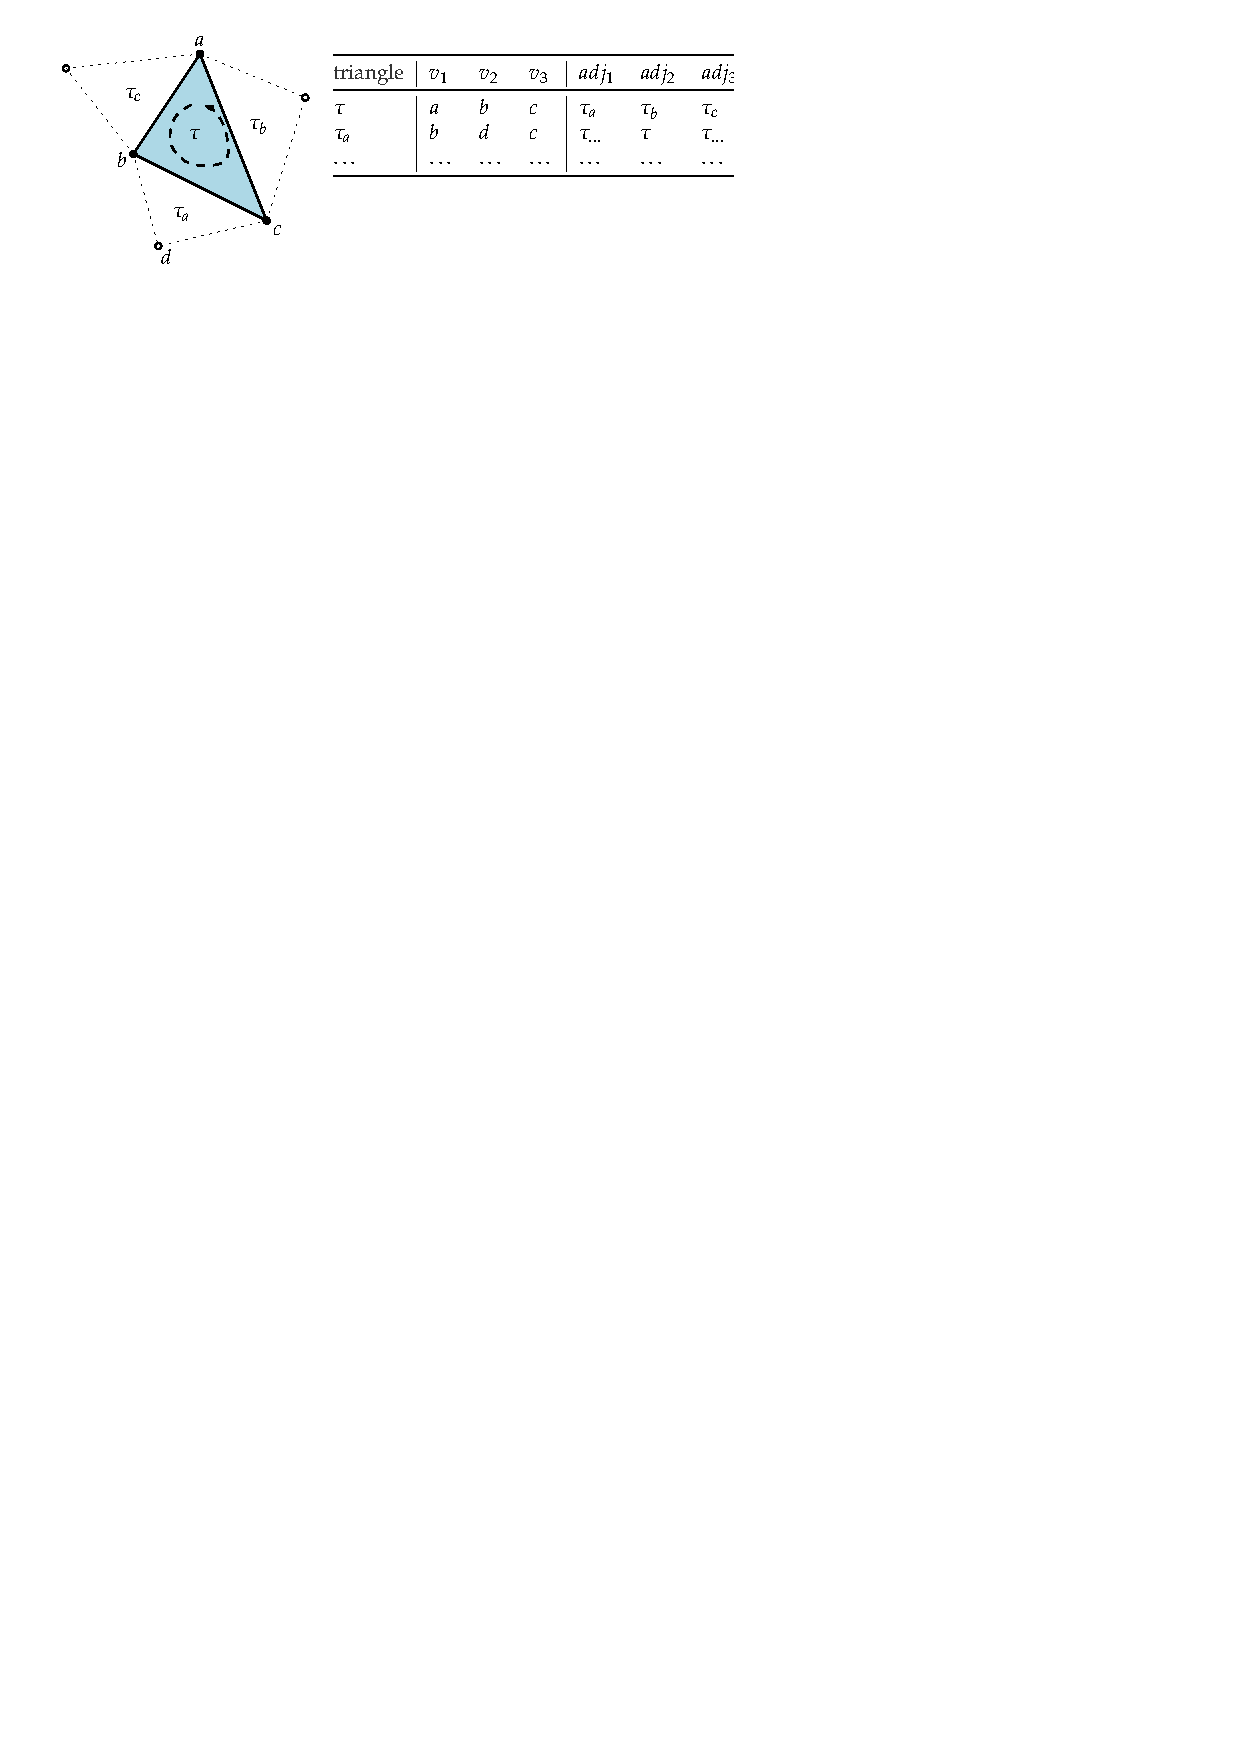
\includegraphics[width=0.95\linewidth]{figs/tr_ds}
  \caption{The triangle-based data structure to store efficiently a triangulation (and the adjacency relationships between the triangles).}
\label{fig:tr_ds}
\end{figure}
considers the triangle as being its atom and stores each triangle with 3 pointers to its vertices and 3 pointers to its adjacent triangles. 




%%%%%%%%%%%%%%%%%%%%%%%%%%%%
\section{Constrained and Conforming Delaunay Triangulations}

Given as input a set $S$ of points and straight-line segments in the plane, different triangulations of $S$ (so that the segments are respected) can be constructed. 
We are mostly interested in the \emph{constrained Delaunay triangulation} (ConsDT) and the \emph{conforming Delaunay triangulation} (ConfDT).
\begin{figure}
  \centering
  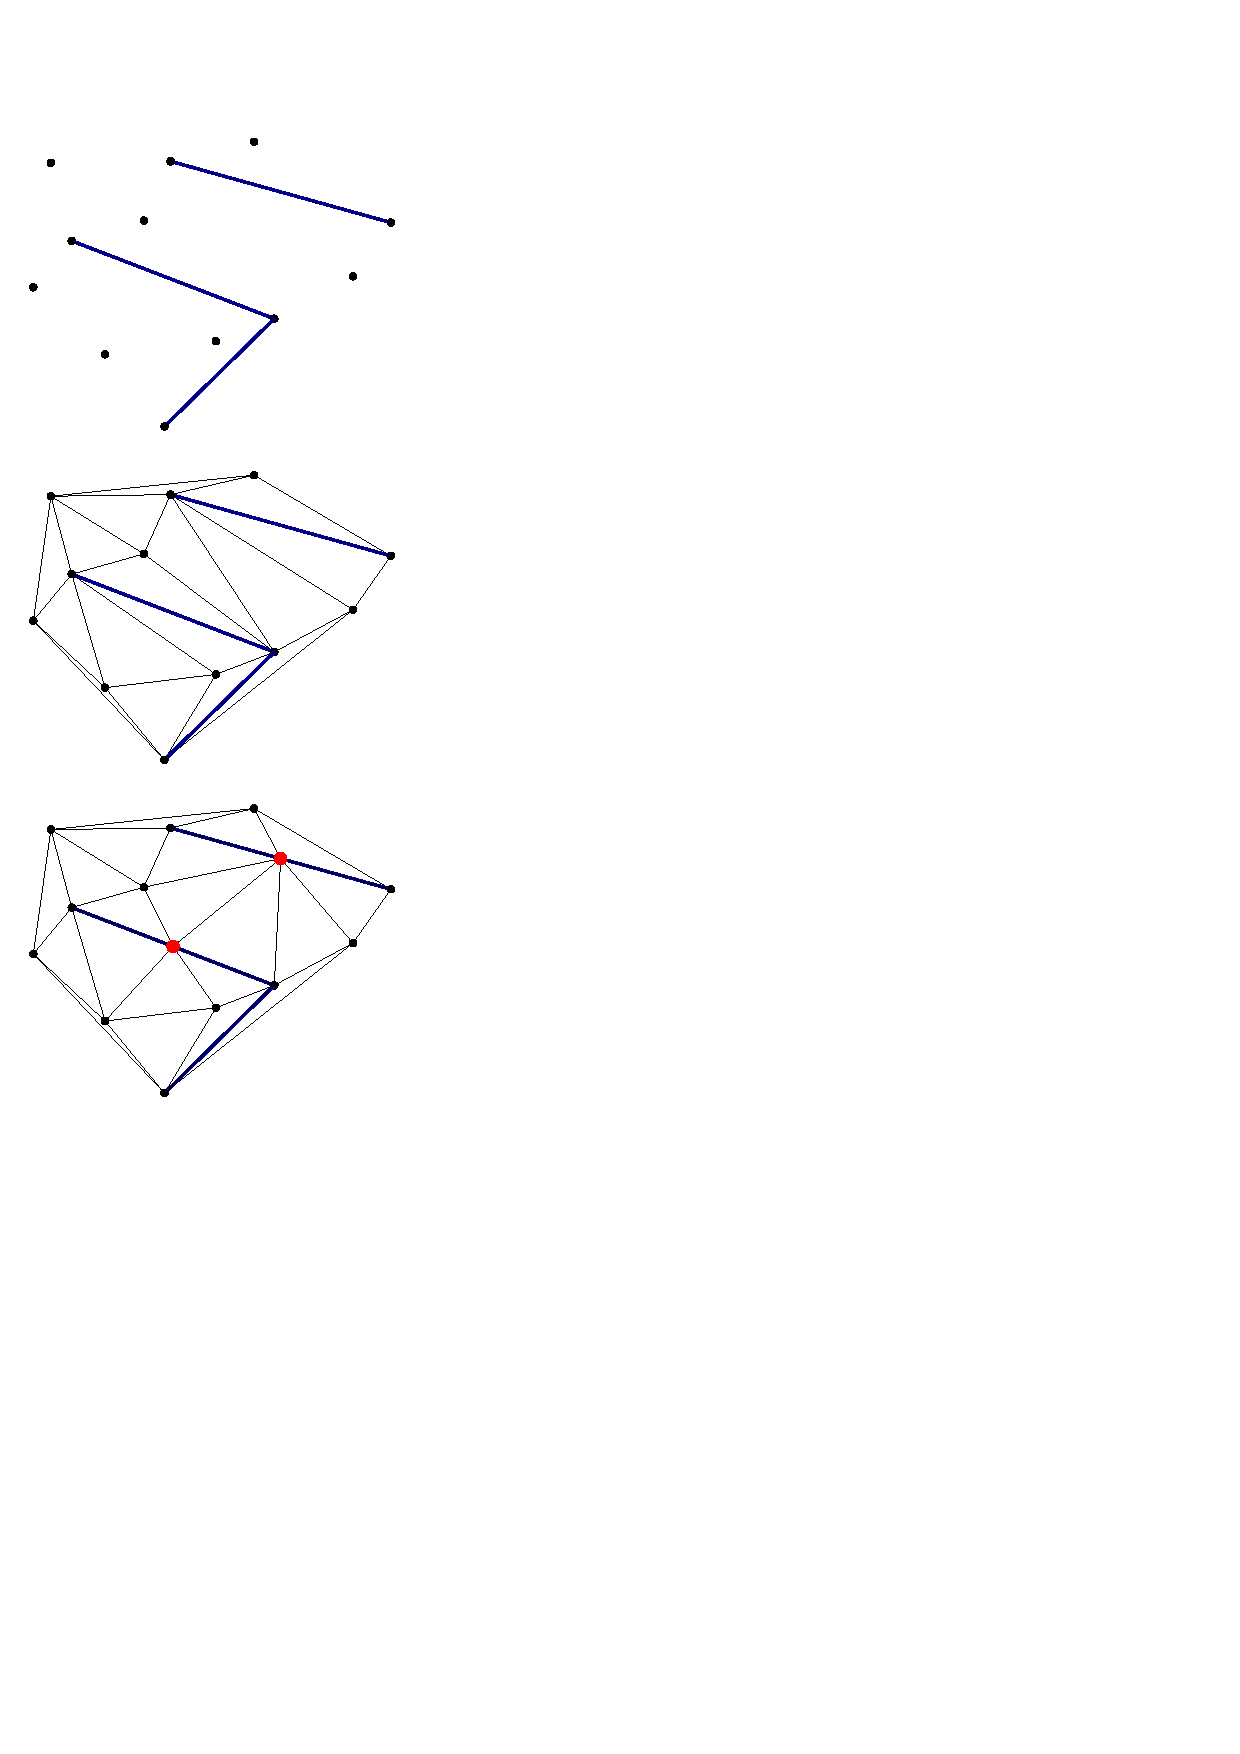
\includegraphics[width=\linewidth]{figs/cdt_example}
  \caption{\textbf{(a)} A a set $S$ of points and straight-line segments. \textbf{(b)} Constrained DT of $S$. \textbf{(c)} Conforming DT of $S$; the Steiner points added are in red.}
\label{fig:cdt_example}
\end{figure}

%%%
%
\paragraph*{Constrained DT (ConsDT).}
Given a set $S$ of points and straight-line segments in $\mathbb{R}^2$, the ConsDT permits us to decompose the convex hull of $S$ into non-overlapping triangles, and every segment of $S$ appears as an edge in ConsDT($S$). 
ConsDT is similar to the Delaunay triangulation, but the triangles in ConsDT are not necessarily Delaunay (\ie\ their circumcircle might contain other points from $S$). 
The empty circumcircle for a ConsDT is less strict: a triangle is Delaunay if its circumcircle contains no other points in $S$ that are \emph{visible} from the triangle.
The constrained segments in $S$ act a visibility blockers. 
Figure~\ref{fig:cdt_buildings} shows one example.
\begin{figure}
  \centering
  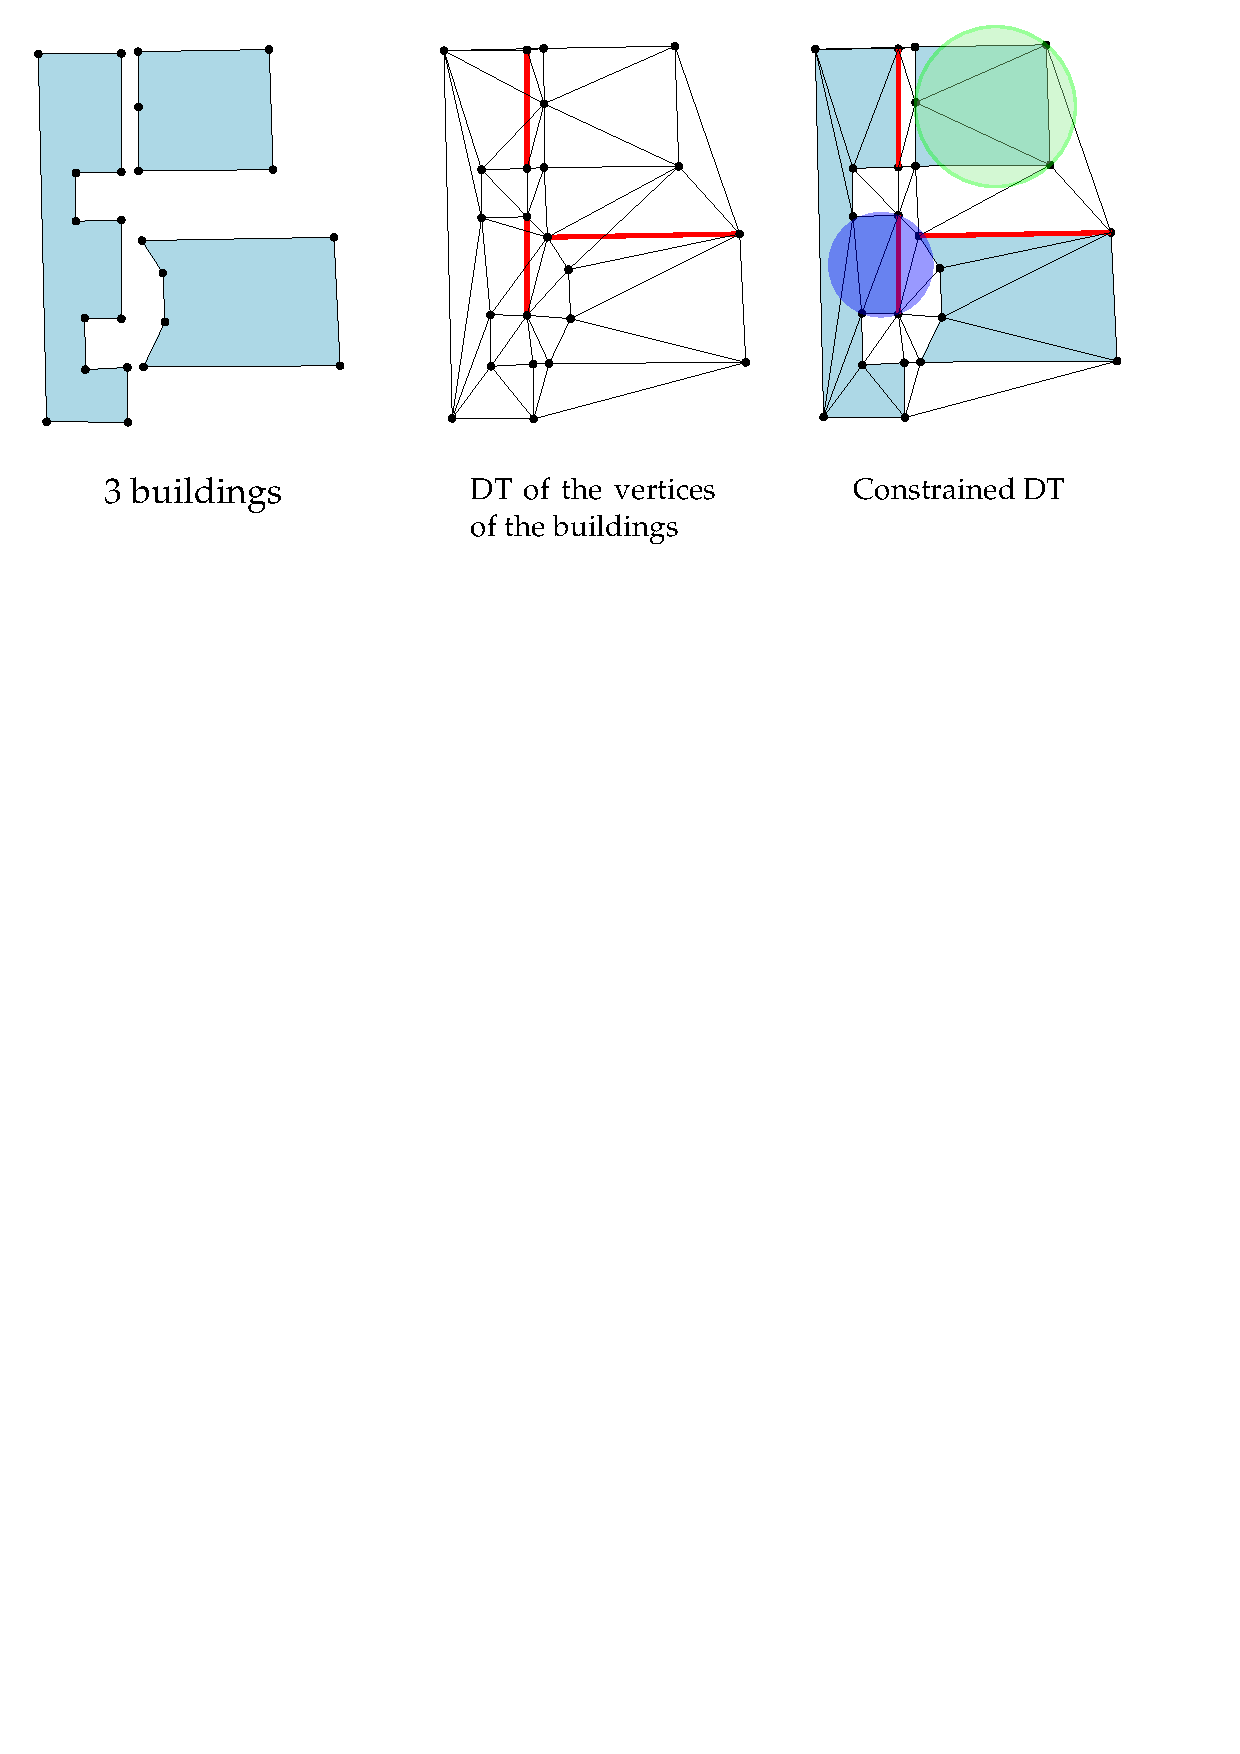
\includegraphics[width=0.95\textwidth]{figs/cdtbuildings}
  \caption{The ConsDT of a set of segments. On the right, the triangle whose circumcircle is green is a Delaunay (no other points in its interior) and so is the triangle whose circumcircle is in blue (there is one point in its interior, but it cannot be seen because of the constrained segment).}
\label{fig:cdt_buildings}
\end{figure}

%

Without going into details about one potential algorithm, one way to construct a ConsDT($S$) is (see Figure~\ref{fig:cdt_steps}:
\begin{figure}
  \centering
  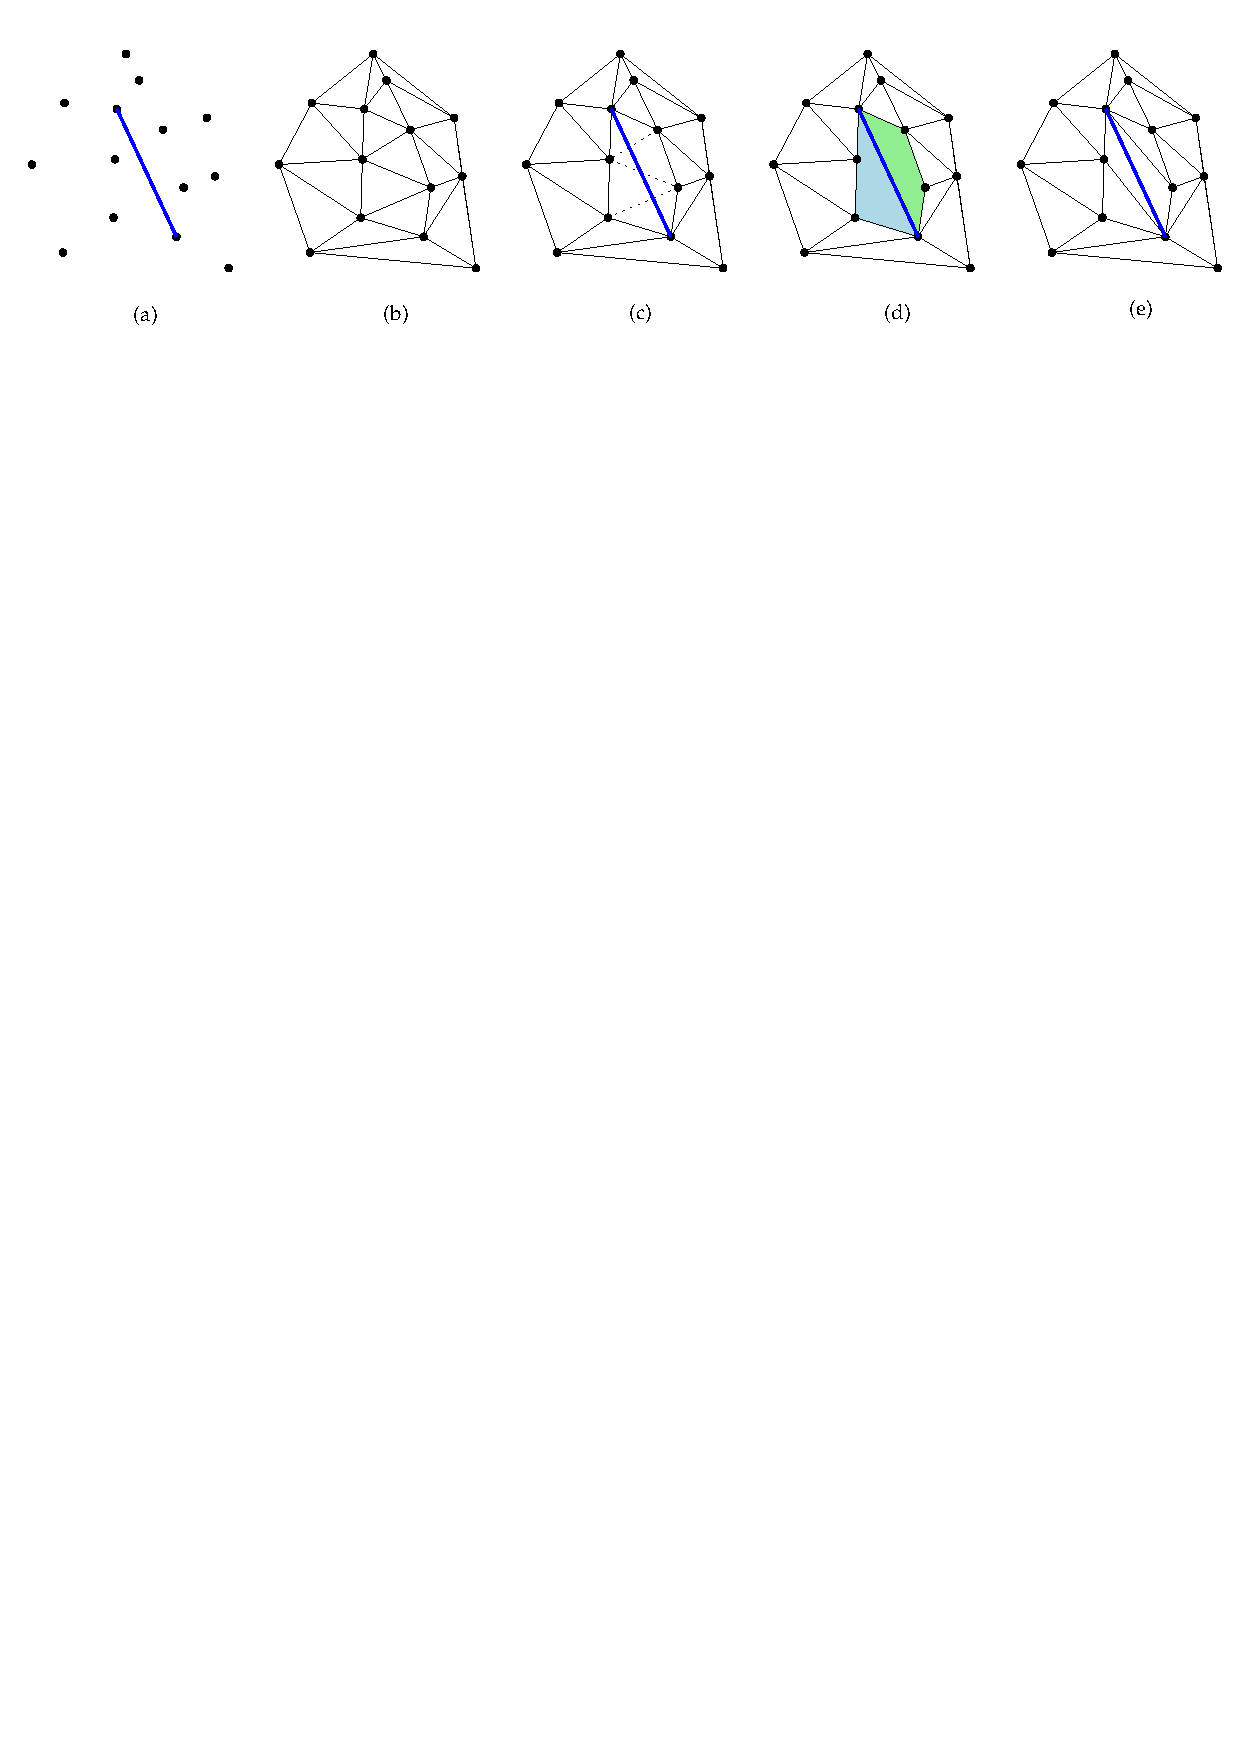
\includegraphics[width=0.95\linewidth]{figs/cdt_steps}
  \caption{Steps to construct a ConsDT.}
\label{fig:cdt_steps}
\end{figure}
\begin{enumerate}
  \item construct DT($S^p$), where $S^p$ is the set containing all the points in $S$ and the end points of the line segments (Figure~\ref{fig:cdt_steps}b)
  \item insert each line segment, each insertion will remove edges from DT($S^p$). In Figure~\ref{fig:cdt_steps}c 3 edges are removed.
  \item this creates 2 polygons that need to be retriangulated, in Figure~\ref{fig:cdt_steps}d there is a blue and a green one.
  \item retriangulate each separately, the Delaunay criterion needs to be verified only for the vertices incident to the triangles incident to the hole/polygon.
\end{enumerate}

%

Observe that the ConsDT can be used to triangulate polygons with holes(see Figure~\ref{fig:cdt_dog}, it suffices to remove the triangle outside the exterior boundary, but inside the convex hull.
\begin{figure}
  \centering
  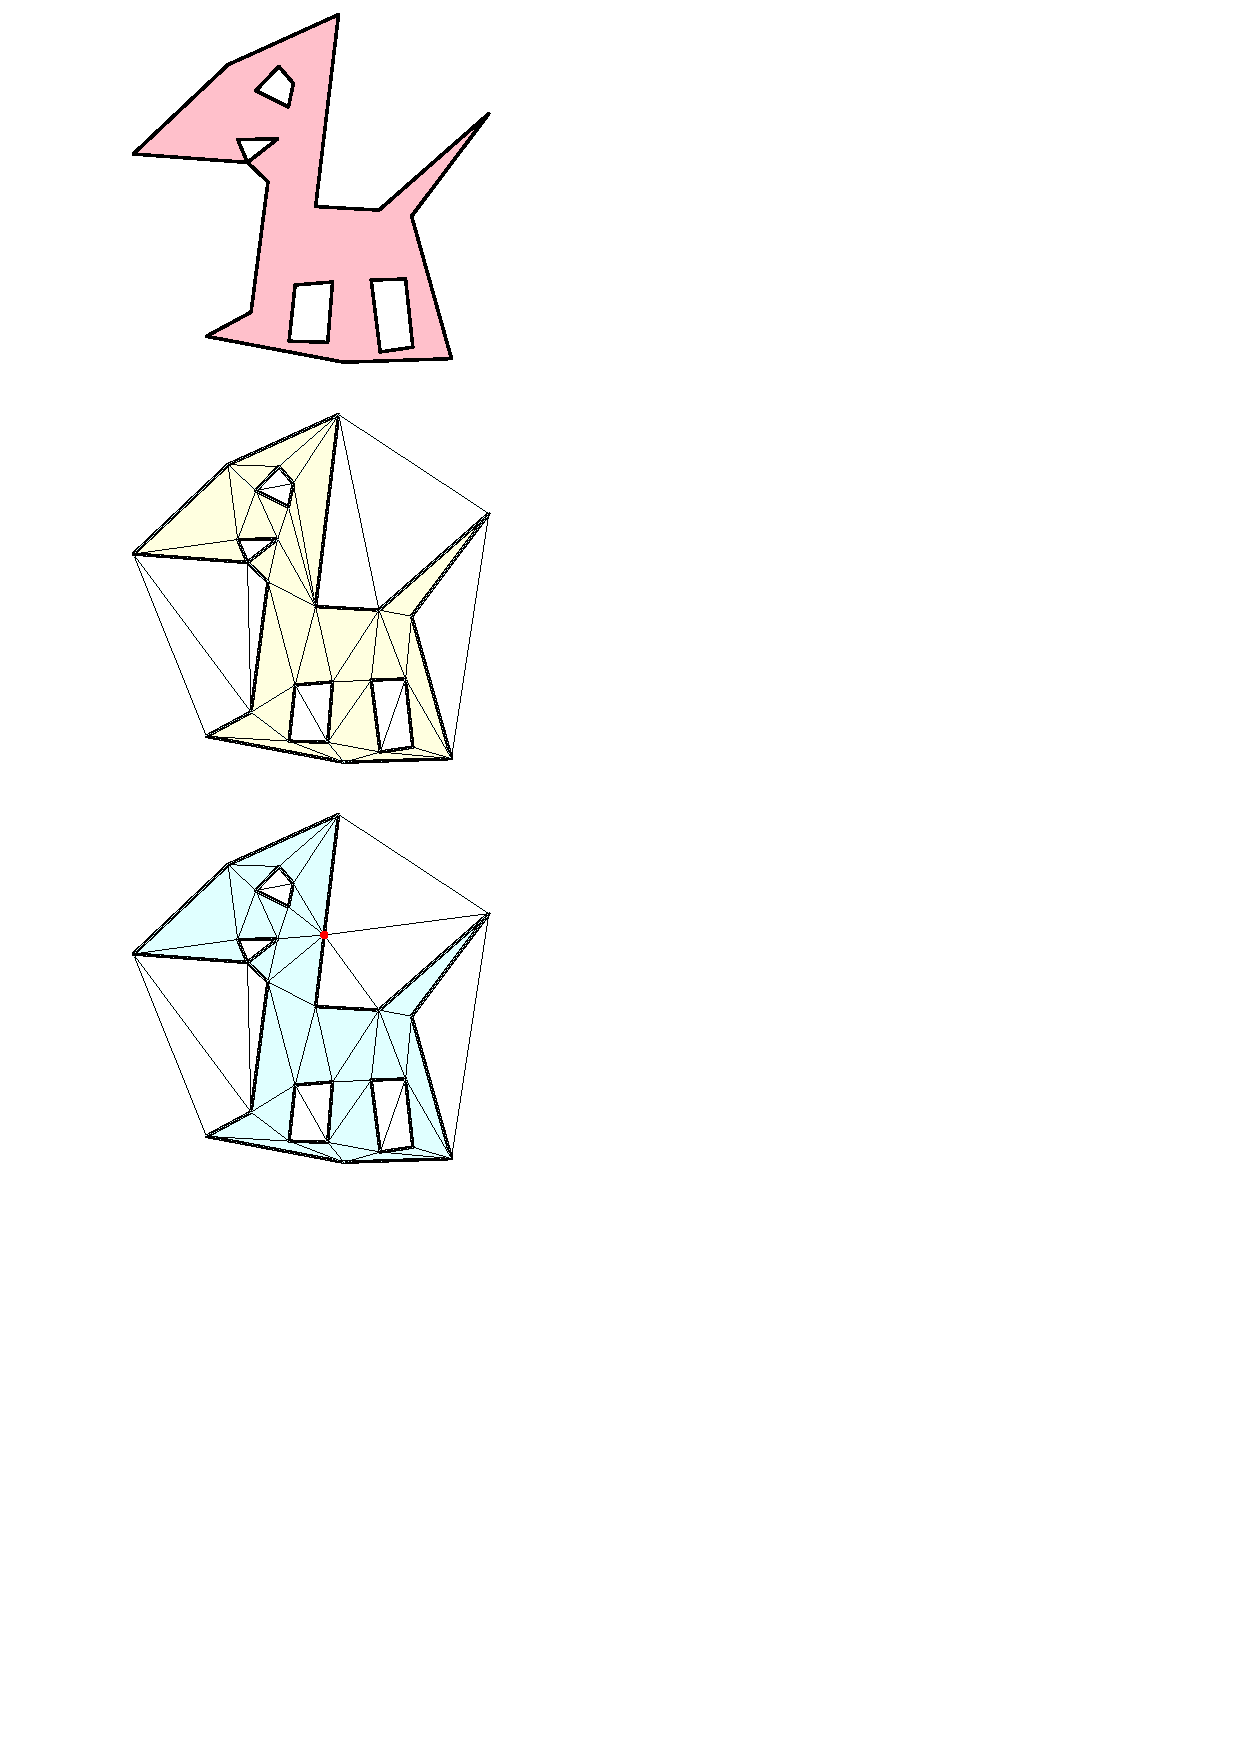
\includegraphics[width=0.6\linewidth]{figs/cdt_dog}
  \caption{\textbf{Left}: One polygon with 4 holes (interior rings). \textbf{Right}: its ConsDT.}
\label{fig:cdt_dog}
\end{figure}


%%%
%
\paragraph*{Conforming DT (ConfDT).}
A ConfDT adds new points to the input $S$ (called \emph{Steiner} points) to ensure that the input segments are present in the triangulation. 
As Figures~\ref{fig:ccdt} and ~\ref{fig:cdt_example}c show, the input straight-line segments will be split into several collinear segments. 
The Steiner points have to be carefully chosen (where to put them is beyond the scope of this course).
\begin{figure}
  \centering
  \begin{subfigure}[b]{0.3\linewidth}
    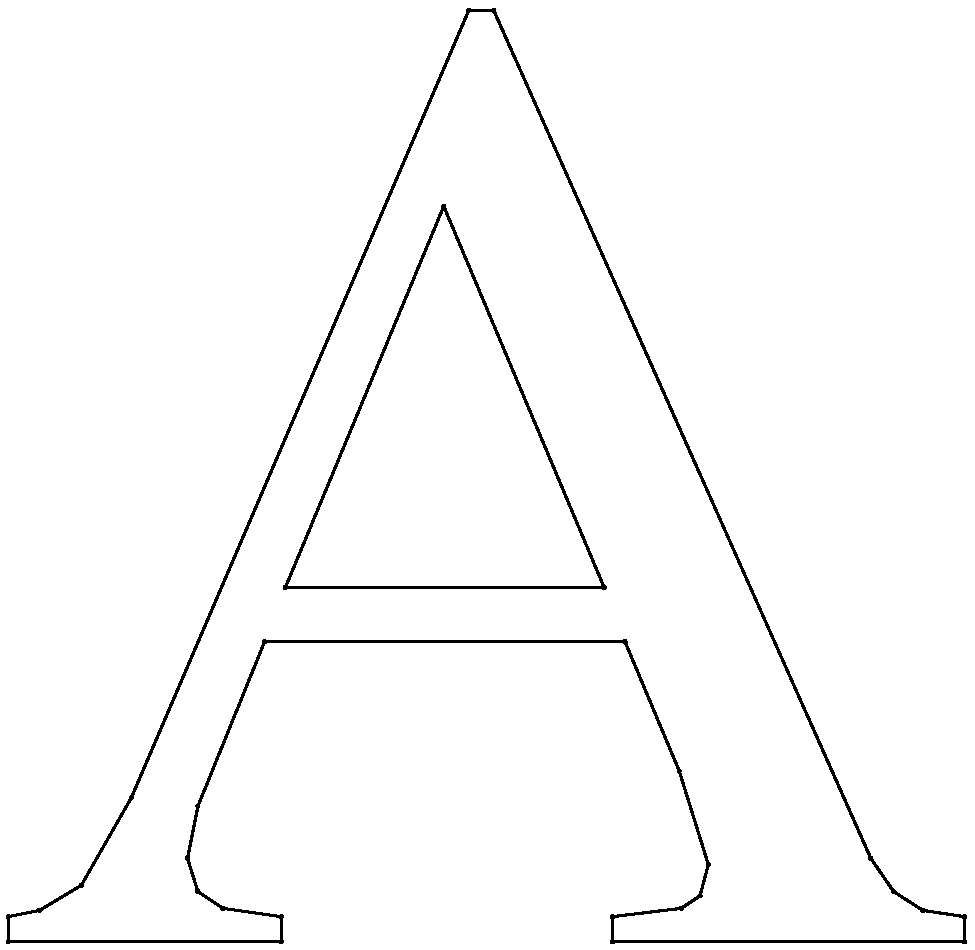
\includegraphics[width=\textwidth]{figs/cdt_input.pdf}
    \caption{}
  \end{subfigure}%
  \qquad
  \begin{subfigure}[b]{0.3\linewidth}
    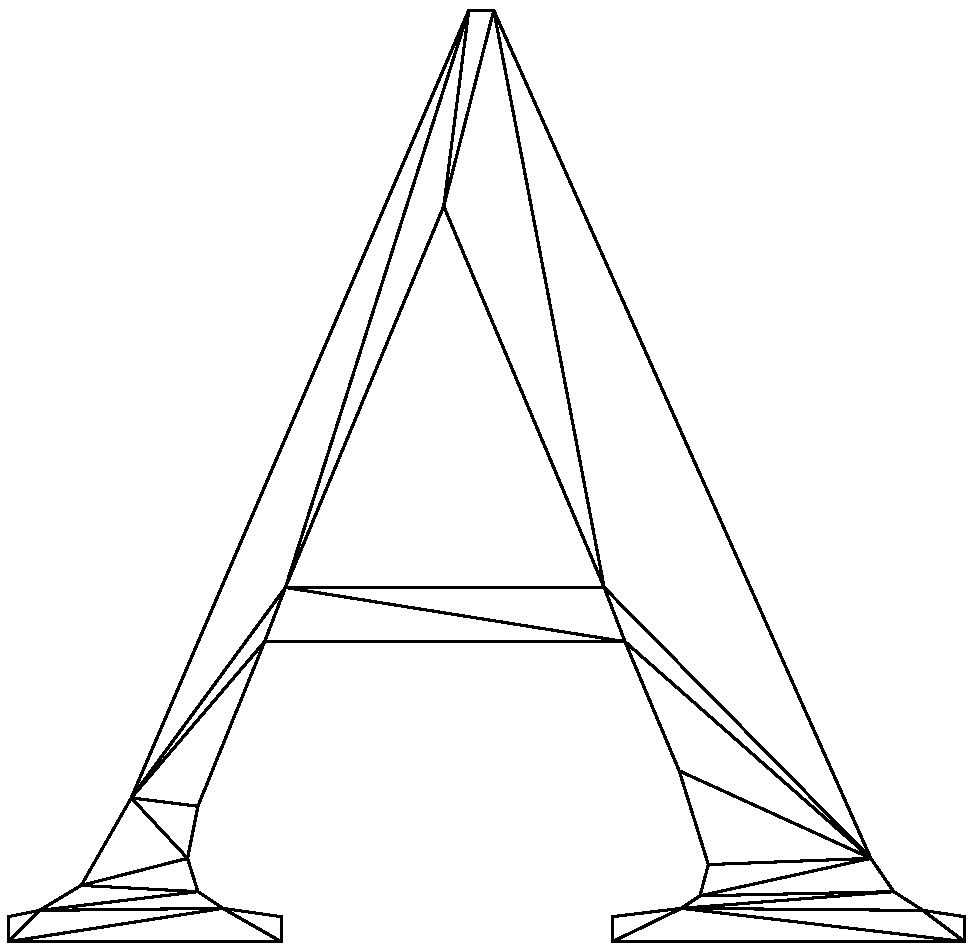
\includegraphics[width=\textwidth]{figs/cdt.pdf}
    \caption{}
  \end{subfigure}%
  \qquad
  \begin{subfigure}[b]{0.3\linewidth}
    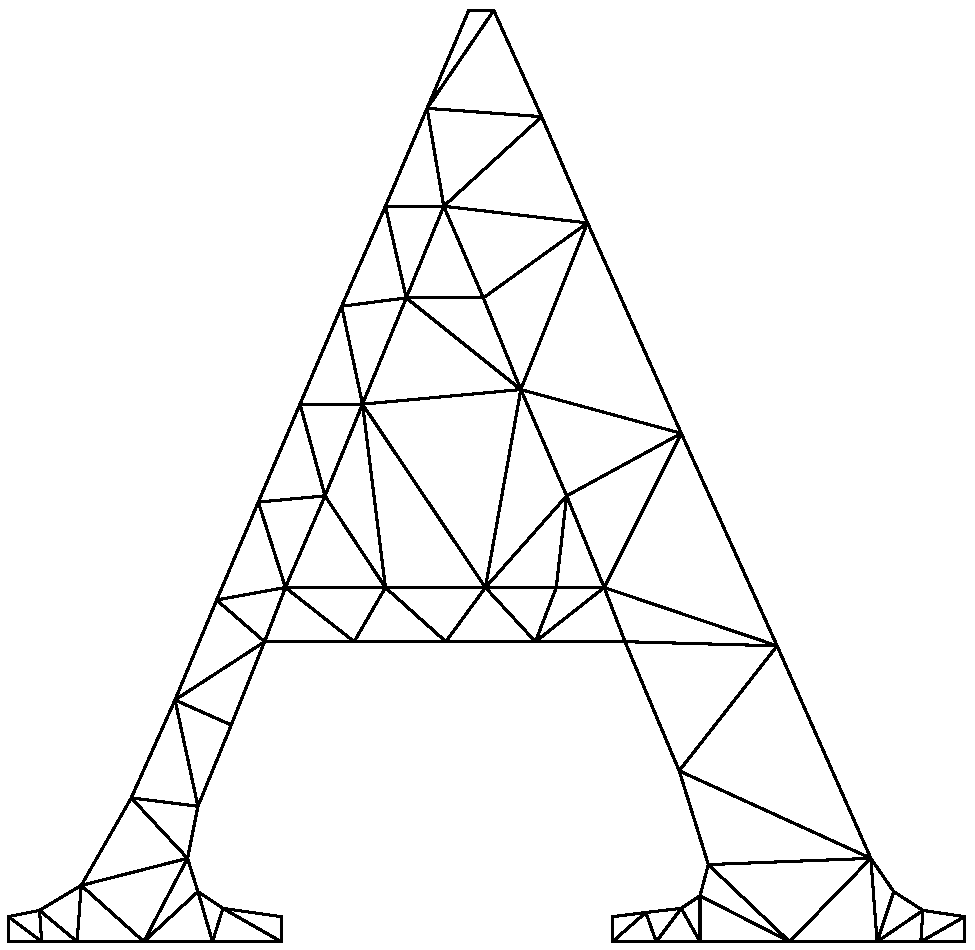
\includegraphics[width=\textwidth]{figs/cdt_conf.pdf}
    \caption{}
  \end{subfigure}%
  \caption{\textbf{(a)} Input polygon (or set of segments). \textbf{(b)} ConsDT of the input. \textbf{(c)} ConfDT of the input.}
\label{fig:ccdt}
\end{figure}
Observe that each triangle in a ConfDT respect the Delaunay criterion, but that more triangles are present. 
If 2 segments are nearly parallel, many points could be necessary (for $m$ segments, up to $m^2$ could be necessary).

%%%%%%%%%%%%%%%%%%%%%%%%%%%%
%%%%%%%%%%%%%%%%%%%%%%%%%%%%
\section{Triangulation of a polygon}

We describe here algorithms to decompose a polygon into non-overlapping triangles (that are not necessarily Delaunay).
While this is not directly related to the modelling of terrains (where we do not have polygons, usually), the topic is relevant in GIS and, as seen below, constrained are often used in terrains.

It is known that any simple polygon (even with holes) can be triangulated without adding new vertices.

%%%
%
\subsection{The trivial case of a convex polygon}

If the polygon to triangulate is convex, then triangulating it is trivial with a \emph{fan-shaped triangulation}.
As shown in Figure~\ref{fig:fanshaped},
\begin{figure}
  \centering
  \begin{subfigure}[b]{0.35\linewidth}
    \centering
    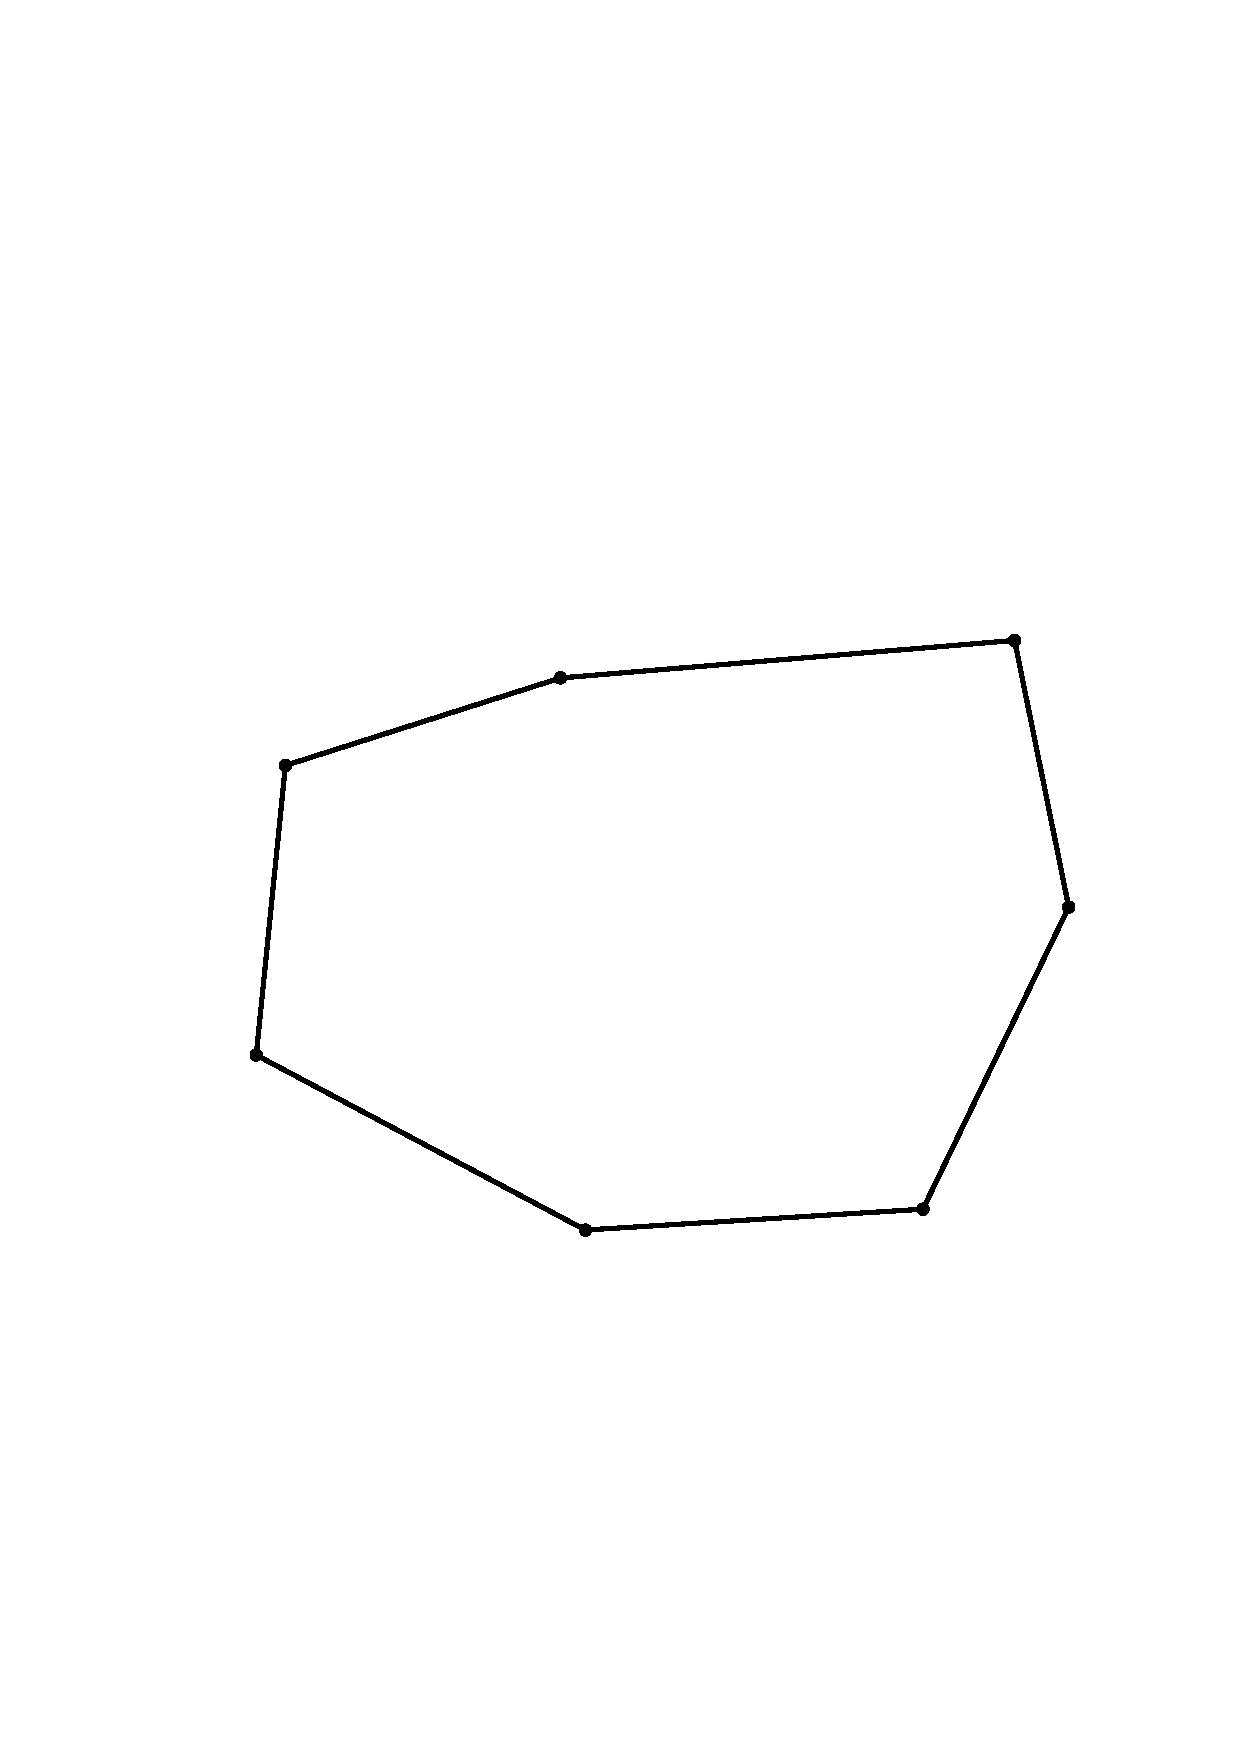
\includegraphics[page=1,width=\textwidth]{figs/fanshaped}
    \caption{}
  \end{subfigure}%
  \qquad
  \begin{subfigure}[b]{0.35\linewidth}
    \centering
    \includegraphics[page=2,width=\textwidth]{figs/fanshaped}
    \caption{}
  \end{subfigure}
\caption{Fan-shaped triangulation of a convex polygon.}
\label{fig:fanshaped}
\end{figure}
the algorithm is simple: starting from an arbitrary vertex $v$ of the polygon $P$, and add edges joining $v$ to all other vertices of $P$, except the previous and next vertices in the ordered boundary of $P$.
A polygon $P$ with $n$ vertices will be triangulated into ($n-2$) triangles.



%%%
%
\subsection{Greedy algorithm for polygons with holes}

A greedy algorithm makes at each step the \emph{locally} optimal choice, and does not look at what has been done before (it never goes back). 
It is very simple to understand and implement, but can yield a very slow implementation.

A greedy algorithm to triangulation a simple polygon $P$ is described in Algorithm~\ref{algo:greedy}.
\begin{algorithm}[tb] 
  \KwIn{Simple polygon $P$ with $n$ vertices}
  \KwOut{Triangulation $\mathcal{T}$ of $P$}
  from the set $D$ of $m=\frac{n(n-3)}{2}$ diagonals of $P$\;
  sort $D$ into ascending order of length $d_1, \ldots, d_m$\;
  triangulation $\mathcal{T} \leftarrow P$\;
  \For{$i \leftarrow 1$ to $m$}
  {
    \If{$d_i$ does not intersect segments in $\mathcal{T}$ AND $d_i$ is an internal diagonal of $P$}
    {
      $\mathcal{T} \leftarrow \mathcal{T} \cup d_i$\;
    }
  }
  \caption{A greedy algorithm to triangulate a simple polygon.}
\label{algo:greedy}
\end{algorithm}
The algorithm basically finds all the potential diagonals for $P$ (all the pairs of vertices), sort them based on their length (ascending length), and at each step of the algorithm the shortest diagonal is inserted if it does not intersect with other already inserted diagonals, and if it is inside $P$. 
Diagonals that have been inserted are never removed. 
When all the possible diagonals have been inserted, each triangle must be constructed by finding 3 segments (boundary of $P$ and diagonals). 
The algorithm is valid for polygon with holes, since all the possible combination of diagonals could be tried.


%%%
%
\subsection{Ear clipping for polygons without holes}

An alternative---and faster---method is by using the ``ear clipping'' algorithm. 
As shown in Figure~\ref{fig:earclipping},
\begin{figure}
  \centering
  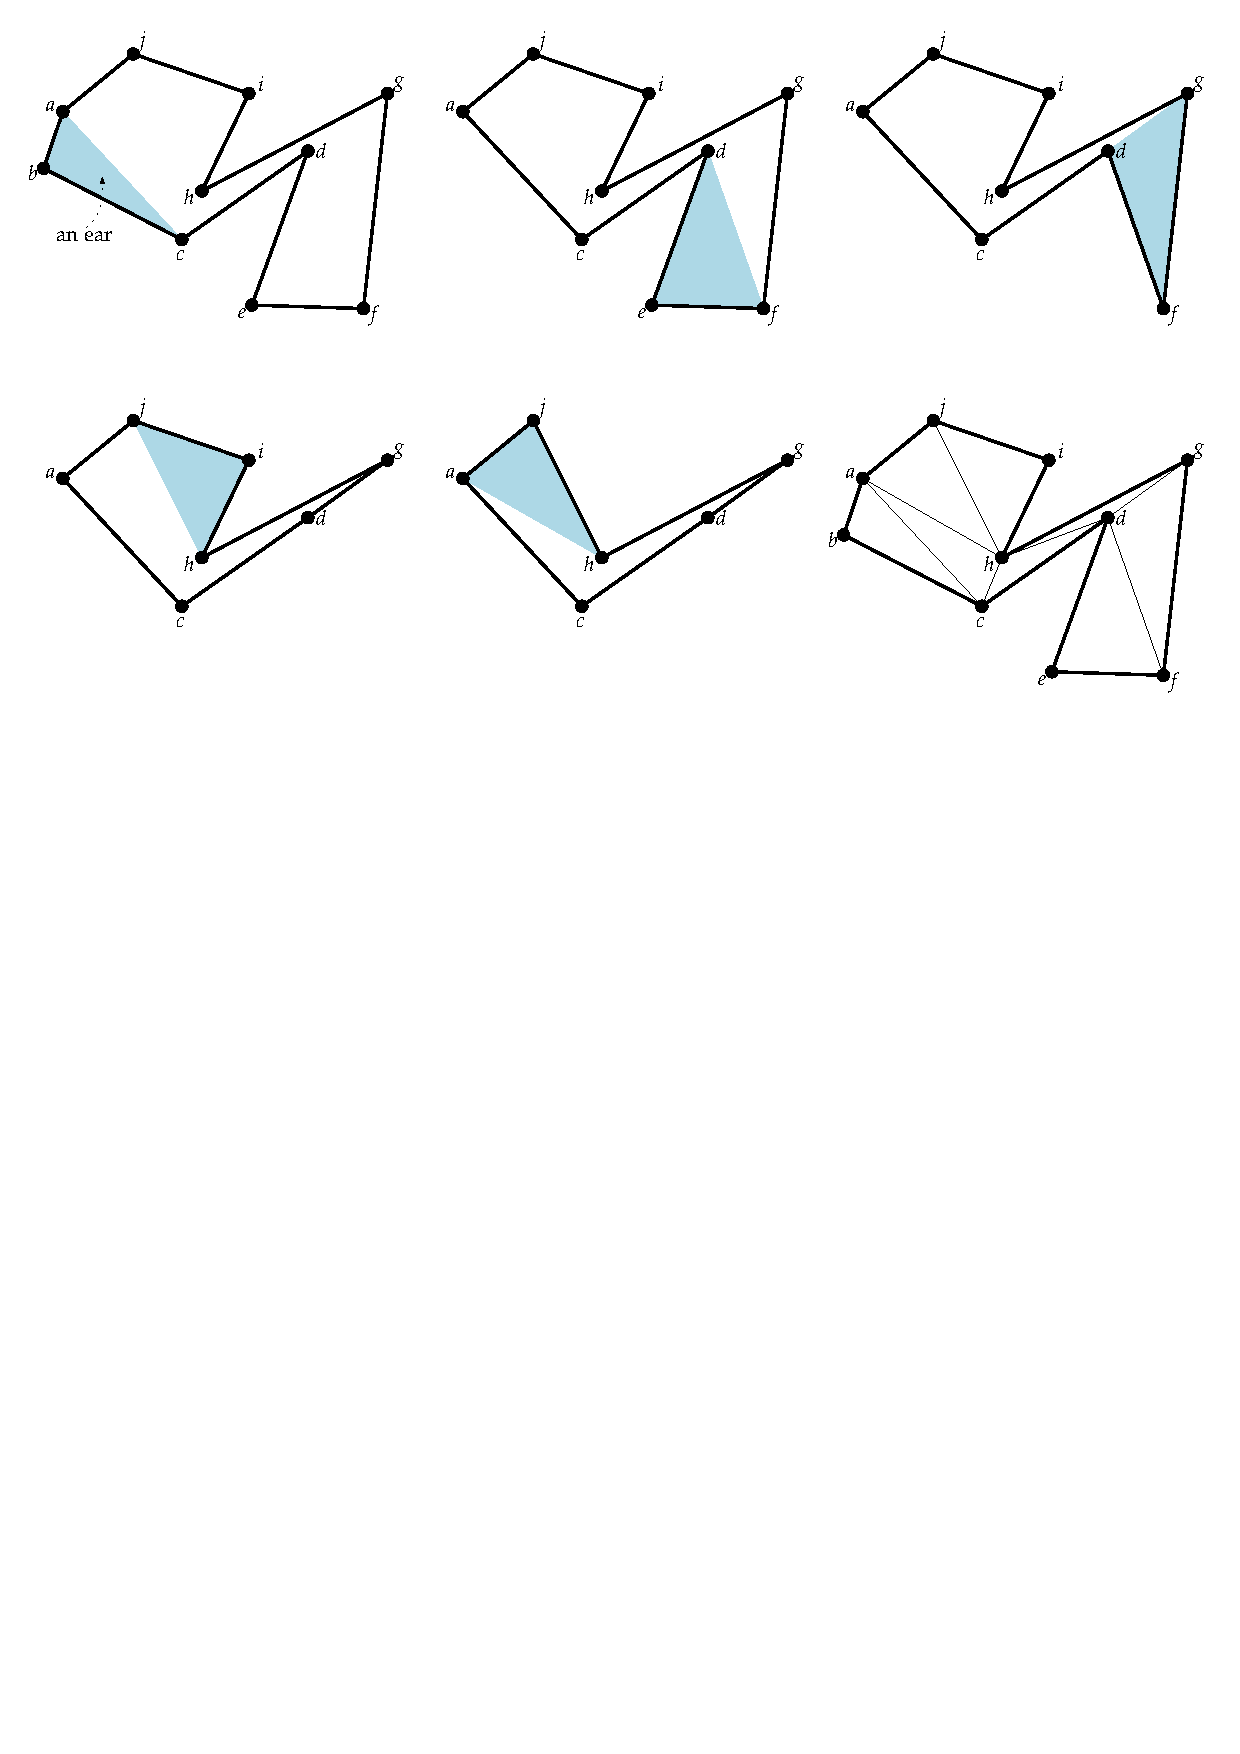
\includegraphics[width=\textwidth]{figs/earclipping}
  \caption{Ear clipping algorithm and the various steps to obtain the triangulation; that last steps are missing.}
\label{fig:earclipping}
\end{figure}
an ear is defined as 3 consecutive points of a polygon forming a triangle; $abc$ is a valid ear of the input polygon $P$, but $cde$ is not (because the triangle is outside the polygon) and neither is $fgh$ (because $d$ is inside the ear).. 
The idea of the ear clipping algorithm is to identify a valid ear, remove it from the polygon and repeat this process (with the modified polygon) until only one triangle is left. 
The implementation is simple: simply keep a list of ordered vertices and each removal of an ear simply removes one vertex (in Figure~\ref{fig:earclipping} at the first step the vertex $b$ is removed).

Observe that this algorithm does not work with polygon having holes.

Finding a valid ear of a simple polygon $P$ is relatively easy: if the points are ordered CCW on the boundary of $P$, then 3 consecutive points must have a positive \Orient; and to verify that the ear is completely inside $P$ the other points of $P$ must be outside that triangle (for instance in Figure~\ref{fig:earclipping} the point $d$ would be inside the triangle $fgh$).


%%%
%
\section{Notes and comments}
\label{sec:notes}

For the construction of the DT, the incremental algorithm we use was first described by \citet{Lawson72-1}.
\citet{Guibas85} describe a divide-and-conquer algorithm, and \citet{Fortune87} a sweep-line one.

The local optimality of a DT, which implies globally optimality in the case of the DT, was proven by \citet{Delaunay34} himself.
The \emph{max-min angle optimality} of the DT was firstly observed by \citet{Sibson78}.
This paraboloic lifting was first observed by \citet{Brown79} (who used a spherical transformation), further described by \citet{Seidel82,Edelsbrunner86}. 


The fact that the DT is computed only in 2D (without taking into account the elevation of the vertices) has been criticised by several as sub-optimal for the modelling of terrain.
To remedy to this, \citet{Dyn90} develop a \emph{data-dependent algorithm}, and \citet{Gudmundsson02} propose using \emph{higher-order} Delaunay triangulations (a modification where the empty circumcircle is also based on the neighbours of the neighbours).
Nevertheless, there are still results stating that the Delaunay triangulation is still the one that minimises the roughness of a surface~\citep{Wang01,Rippa90}

% TODO : complete this: uniqueness of the DT
% If the input points of the DT are not in general position, it is still possible to obtain a unique DT\@.
% This however means that 

The Algorithm~\ref{algo:greedy}, is taken from \citet[p. 202]{Worboys04}.

\citet{Shewchuk97} shows that while the triangle-based data structure requires twice as much code as with the quad-edge (to store and construct a ConsDT), the result is that the code runs twice as fast and the memory requirement as about 2X less.
CGAL (\url{https://www.cgal.org/}), among many others, uses the triangle-based data structure.

